\documentclass[11pt,a4paper,twocolumn]{article}

\usepackage[utf8]{inputenc}
\usepackage[margin=20mm]{geometry}
\usepackage{times}
\usepackage{latexsym}
\usepackage{amsmath,amssymb}
\usepackage{graphicx}
\usepackage{booktabs}
\usepackage{multirow}
\usepackage{microtype}
\usepackage{xcolor}
\usepackage{float}
\usepackage{url}
\usepackage[hidelinks]{hyperref}

\title{\textbf{Classifying Consumer Financial Complaints by Product Category:\\A Comparative Study of Text Representations, Neural Architectures, and Causal Decoder Small Language Models (Qwen2.5)}}

\author{
  \textbf{Nabil Ishmam} \quad \textbf{Quazi Unjurn Daniel} \quad \textbf{Shoumodip Paul} \quad \textbf{Afnan Mojumder} \\
  Department of Computer Science and Engineering, BRAC University \\
  \texttt{\{nabil.ishmam, quazi.unjurn.daniel, shoumodip.paul, afnan.mojumder\}@g.bracu.ac.bd}
}

\date{}

\begin{document}

\maketitle

\begin{abstract}
We classify 2.02 million U.S. Consumer Financial Protection Bureau (CFPB) complaint narratives into nine consolidated product categories, benchmarking eleven architectures spanning four distinct NLP paradigms: classical bag-of-words over sublinear TF-IDF, six recurrent neural networks over domain Word2Vec CBOW embeddings, a fine-tuned BERT Base bidirectional transformer, and a modern 1.54B parameter Causal Decoder Small Language Model (\textbf{Qwen2.5-1.5B}) adapted via Parameter-Efficient Fine-Tuning (LoRA, $r=16$). All models are evaluated on an identical 303,213-document held-out test split under a rigorous zero-leakage protocol. \textbf{BERT Base} attains peak overall performance (\textbf{Test Macro F1 = 0.7738, Accuracy = 86.51\%}), while \textbf{Qwen2.5 (1.5B LoRA)} achieves \textbf{0.7427 Macro F1 and 82.84\% Accuracy} by updating only 1.18\% (18.48M) of its parameters. Qwen2.5 outperforms all six recurrent architectures (Bi-GRU 0.7248, Bi-LSTM 0.7169) by avoiding sequential memory bottlenecks, but incurs an inference latency penalty (62.16 ms vs. 4.82 ms for BERT and 0.10 ms for Logistic Regression). Additionally, our novelty investigation into class imbalance (52.9:1 skew) reveals that SMOTE oversampling dramatically rescues minority-class F1 for tree ensembles (+0.2809 gain on Random Forest), whereas linear and deep models perform best without synthetic oversampling.
\end{abstract}

\section{Introduction}
The Consumer Financial Protection Bureau (CFPB) processes hundreds of thousands of consumer complaints annually, maintaining the largest public financial grievance database in the United States ($>2.02$ million complaints). Automated multi-class routing is critical for regulatory triage, compliance enforcement, and consumer risk monitoring. 

However, real-world complaint streams exhibit acute domain challenges:
\begin{enumerate}
    \item \textbf{Extreme Class Imbalance:} A 52.9:1 ratio between the majority category (\textit{Credit reporting}, 59.60\%) and the rarest category (\textit{Payday / personal loans}, 1.13\%).
    \item \textbf{Linguistic Complexity:} High lexical overlap among financial products, verbose legal phrasing, and pervasive PII redactions (\texttt{XXXX}).
    \item \textbf{Architectural Trade-offs:} Balancing classification expressivity against computational throughput in enterprise deployment.
\end{enumerate}

In this study, we provide a unified comparative investigation across four paradigms: (i) Classical ML with sparse n-gram TF-IDF; (ii) Recurrent neural architectures (SimpleRNN, GRU, LSTM, and their bidirectional variants) over domain Word2Vec embeddings; (iii) Bidirectional contextual pretrained encoders (BERT Base); and (iv) Modern autoregressive causal decoders (\textbf{Qwen2.5-1.5B}) fine-tuned via Low-Rank Adaptation (LoRA).

\section{Related Work}
\paragraph{Classical NLP Baselines.} Sublinear TF-IDF term weighting \cite{sparck1972statistical} paired with linear classifiers remains an extraordinarily competitive baseline for high-dimensional topical classification \cite{joachims1998text}, while Multinomial Naive Bayes provides instant linear-time estimation \cite{mccallum1998comparison}. Random Forests extend to sparse matrices but are vulnerable to skewed class priors \cite{breiman2001random}.

\paragraph{Recurrent Neural Networks.} Sequential recurrent architectures suffer from vanishing and exploding gradients over long documents \cite{elman1990finding}. Gated mechanisms—LSTM \cite{hochreiter1997long} and GRU \cite{cho2014learning}—mitigate degradation by learning adaptive memory retention gates, augmented by bidirectional processing \cite{schuster1997bidirectional} and distributed continuous representations \cite{mikolov2013efficient}.

\paragraph{Transformers \& Causal Decoder SLMs.} Bidirectional Encoder Representations from Transformers (BERT; \cite{devlin2019bert}) established the standard for contextual sentence encoding via unconstrained masked language modeling. Recently, modern Small Language Models (SLMs) such as the Qwen2.5 family \cite{yang2024qwen2} have demonstrated exceptional linguistic reasoning via dense multi-head self-attention. Low-Rank Adaptation (LoRA; \cite{hu2021lora}) enables parameter-efficient adaptation of billion-parameter decoder models by decomposing weight updates into low-rank intrinsic matrices ($W = W_0 + B A$), freezing 98.8\% of base weights.

\section{Corpus \& Preprocessing Pipeline}

\begin{figure}[t]
    \centering
    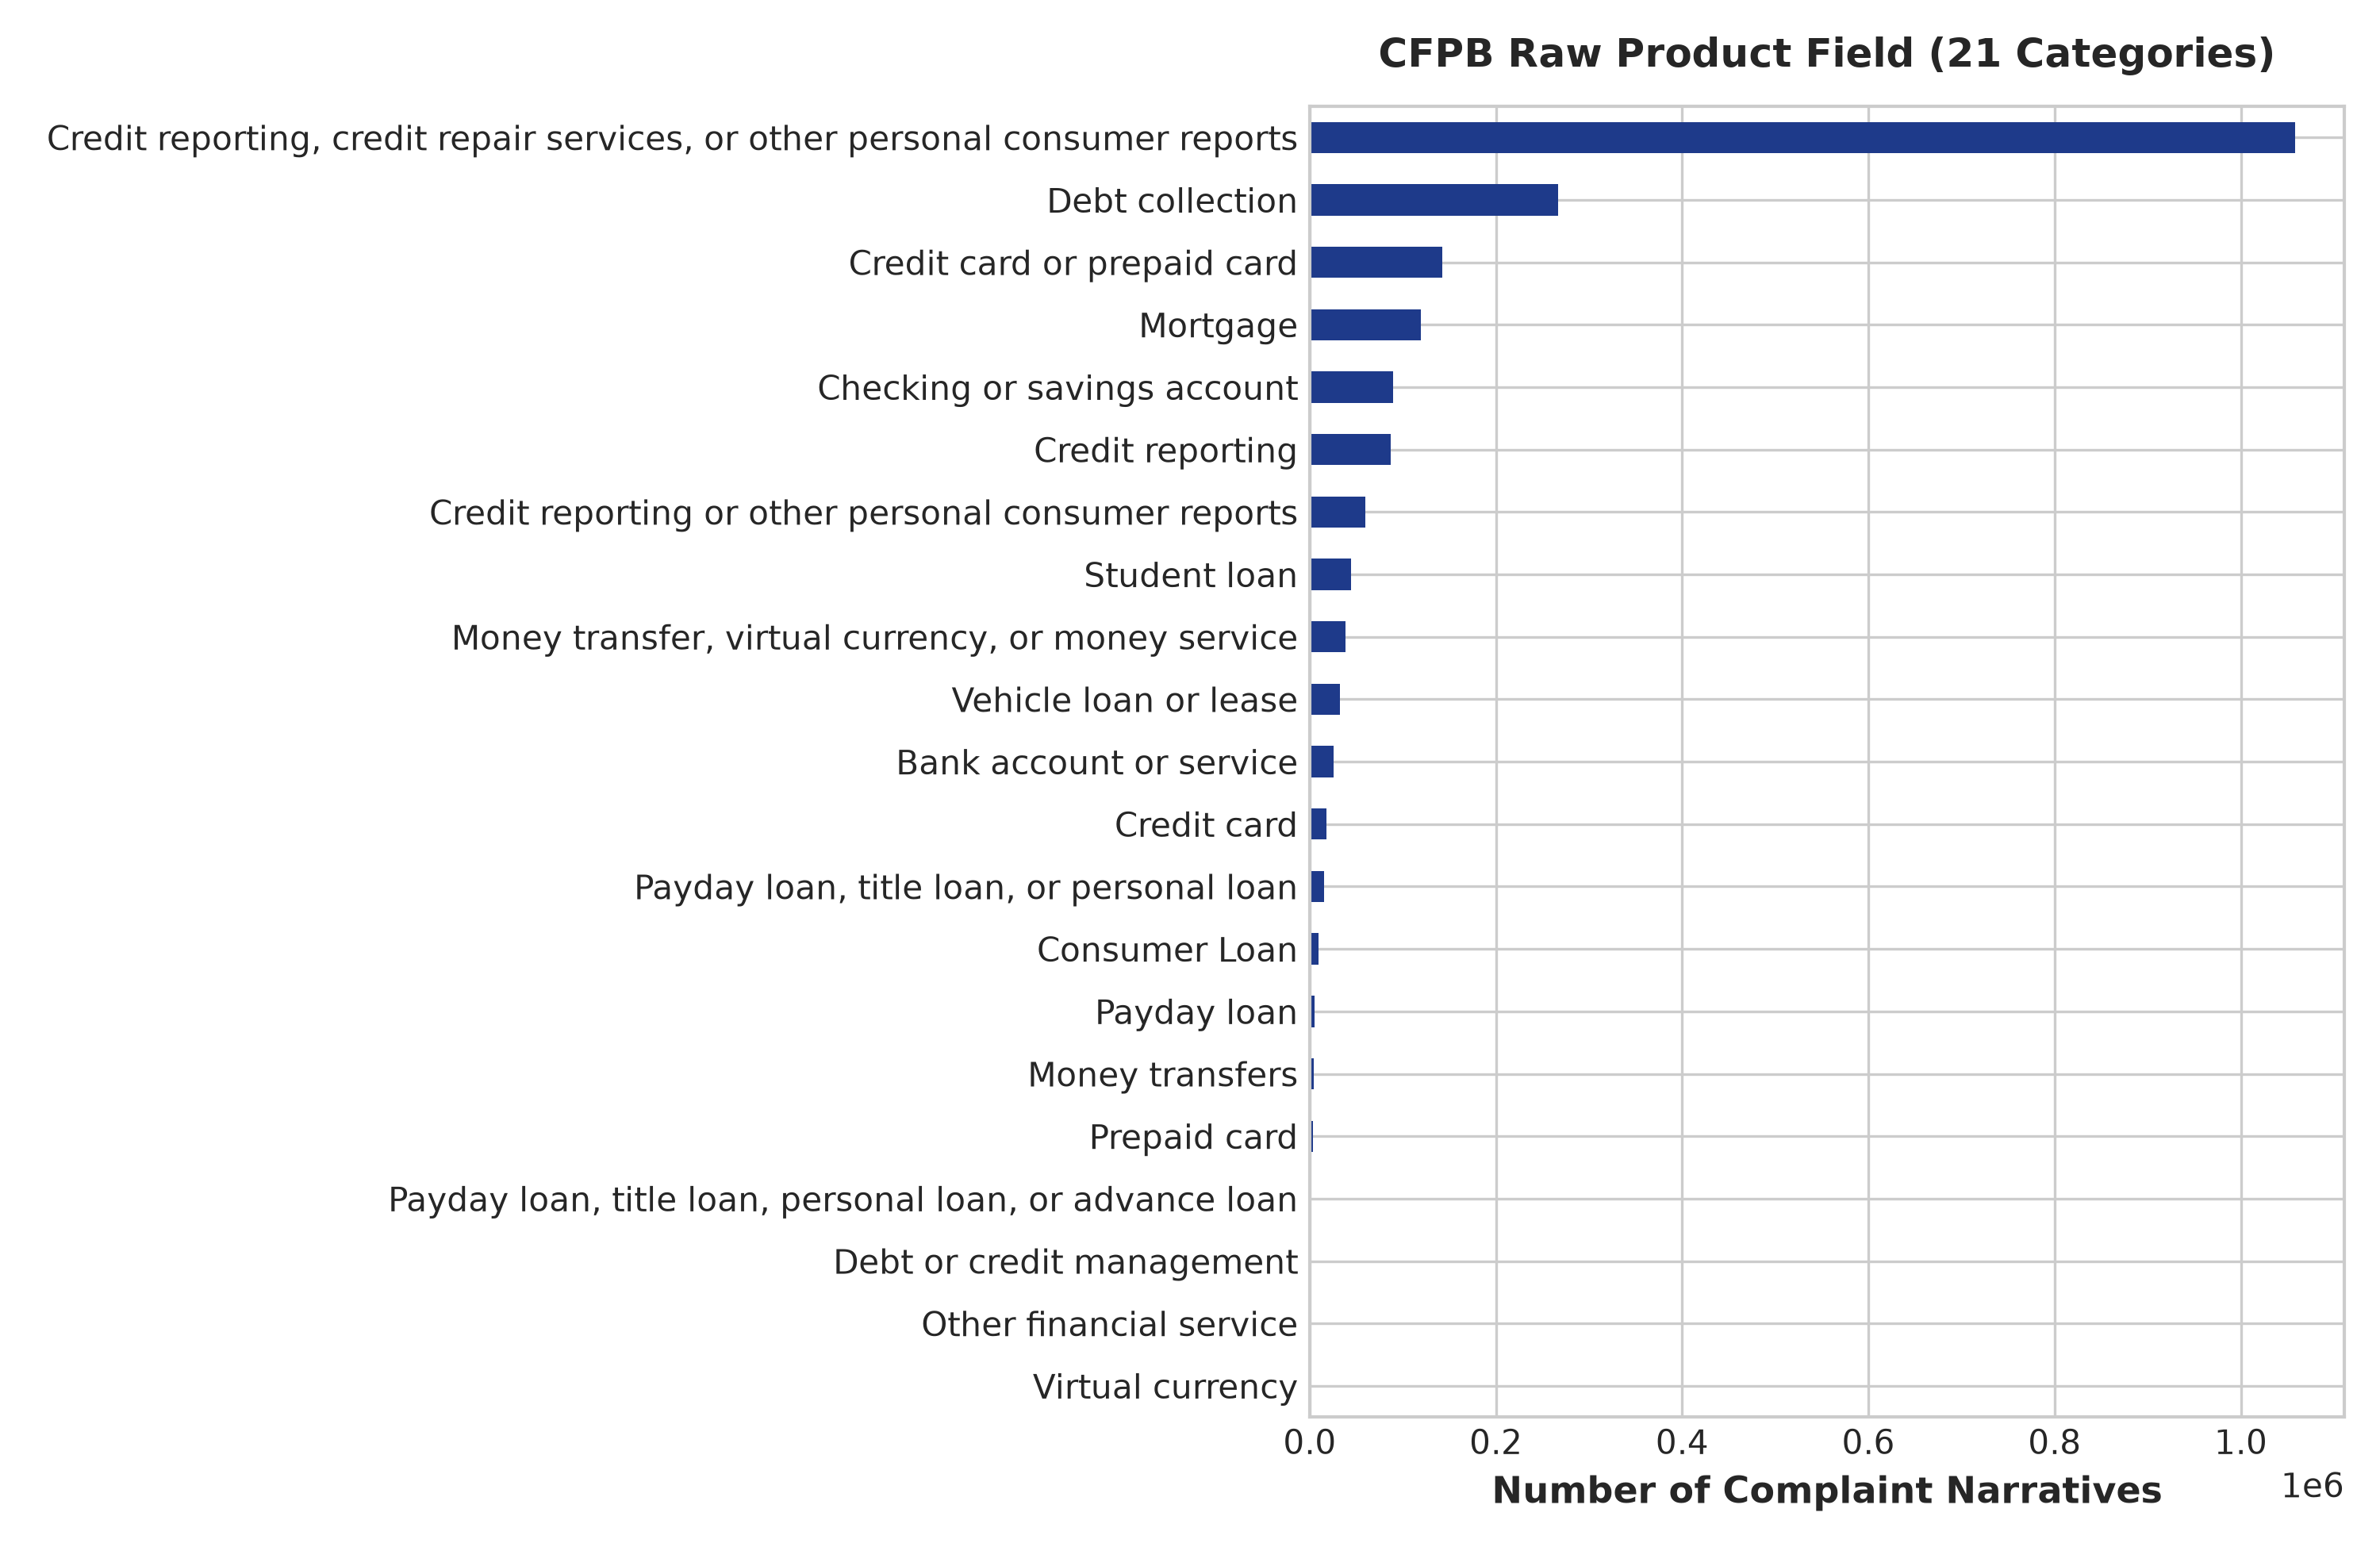
\includegraphics[width=\columnwidth]{figures/fig1_raw_products.png}
    \caption{Distribution of raw CFPB product categories (21 classes) prior to taxonomic consolidation.}
    \label{fig:raw_products}
\end{figure}

\begin{figure}[t]
    \centering
    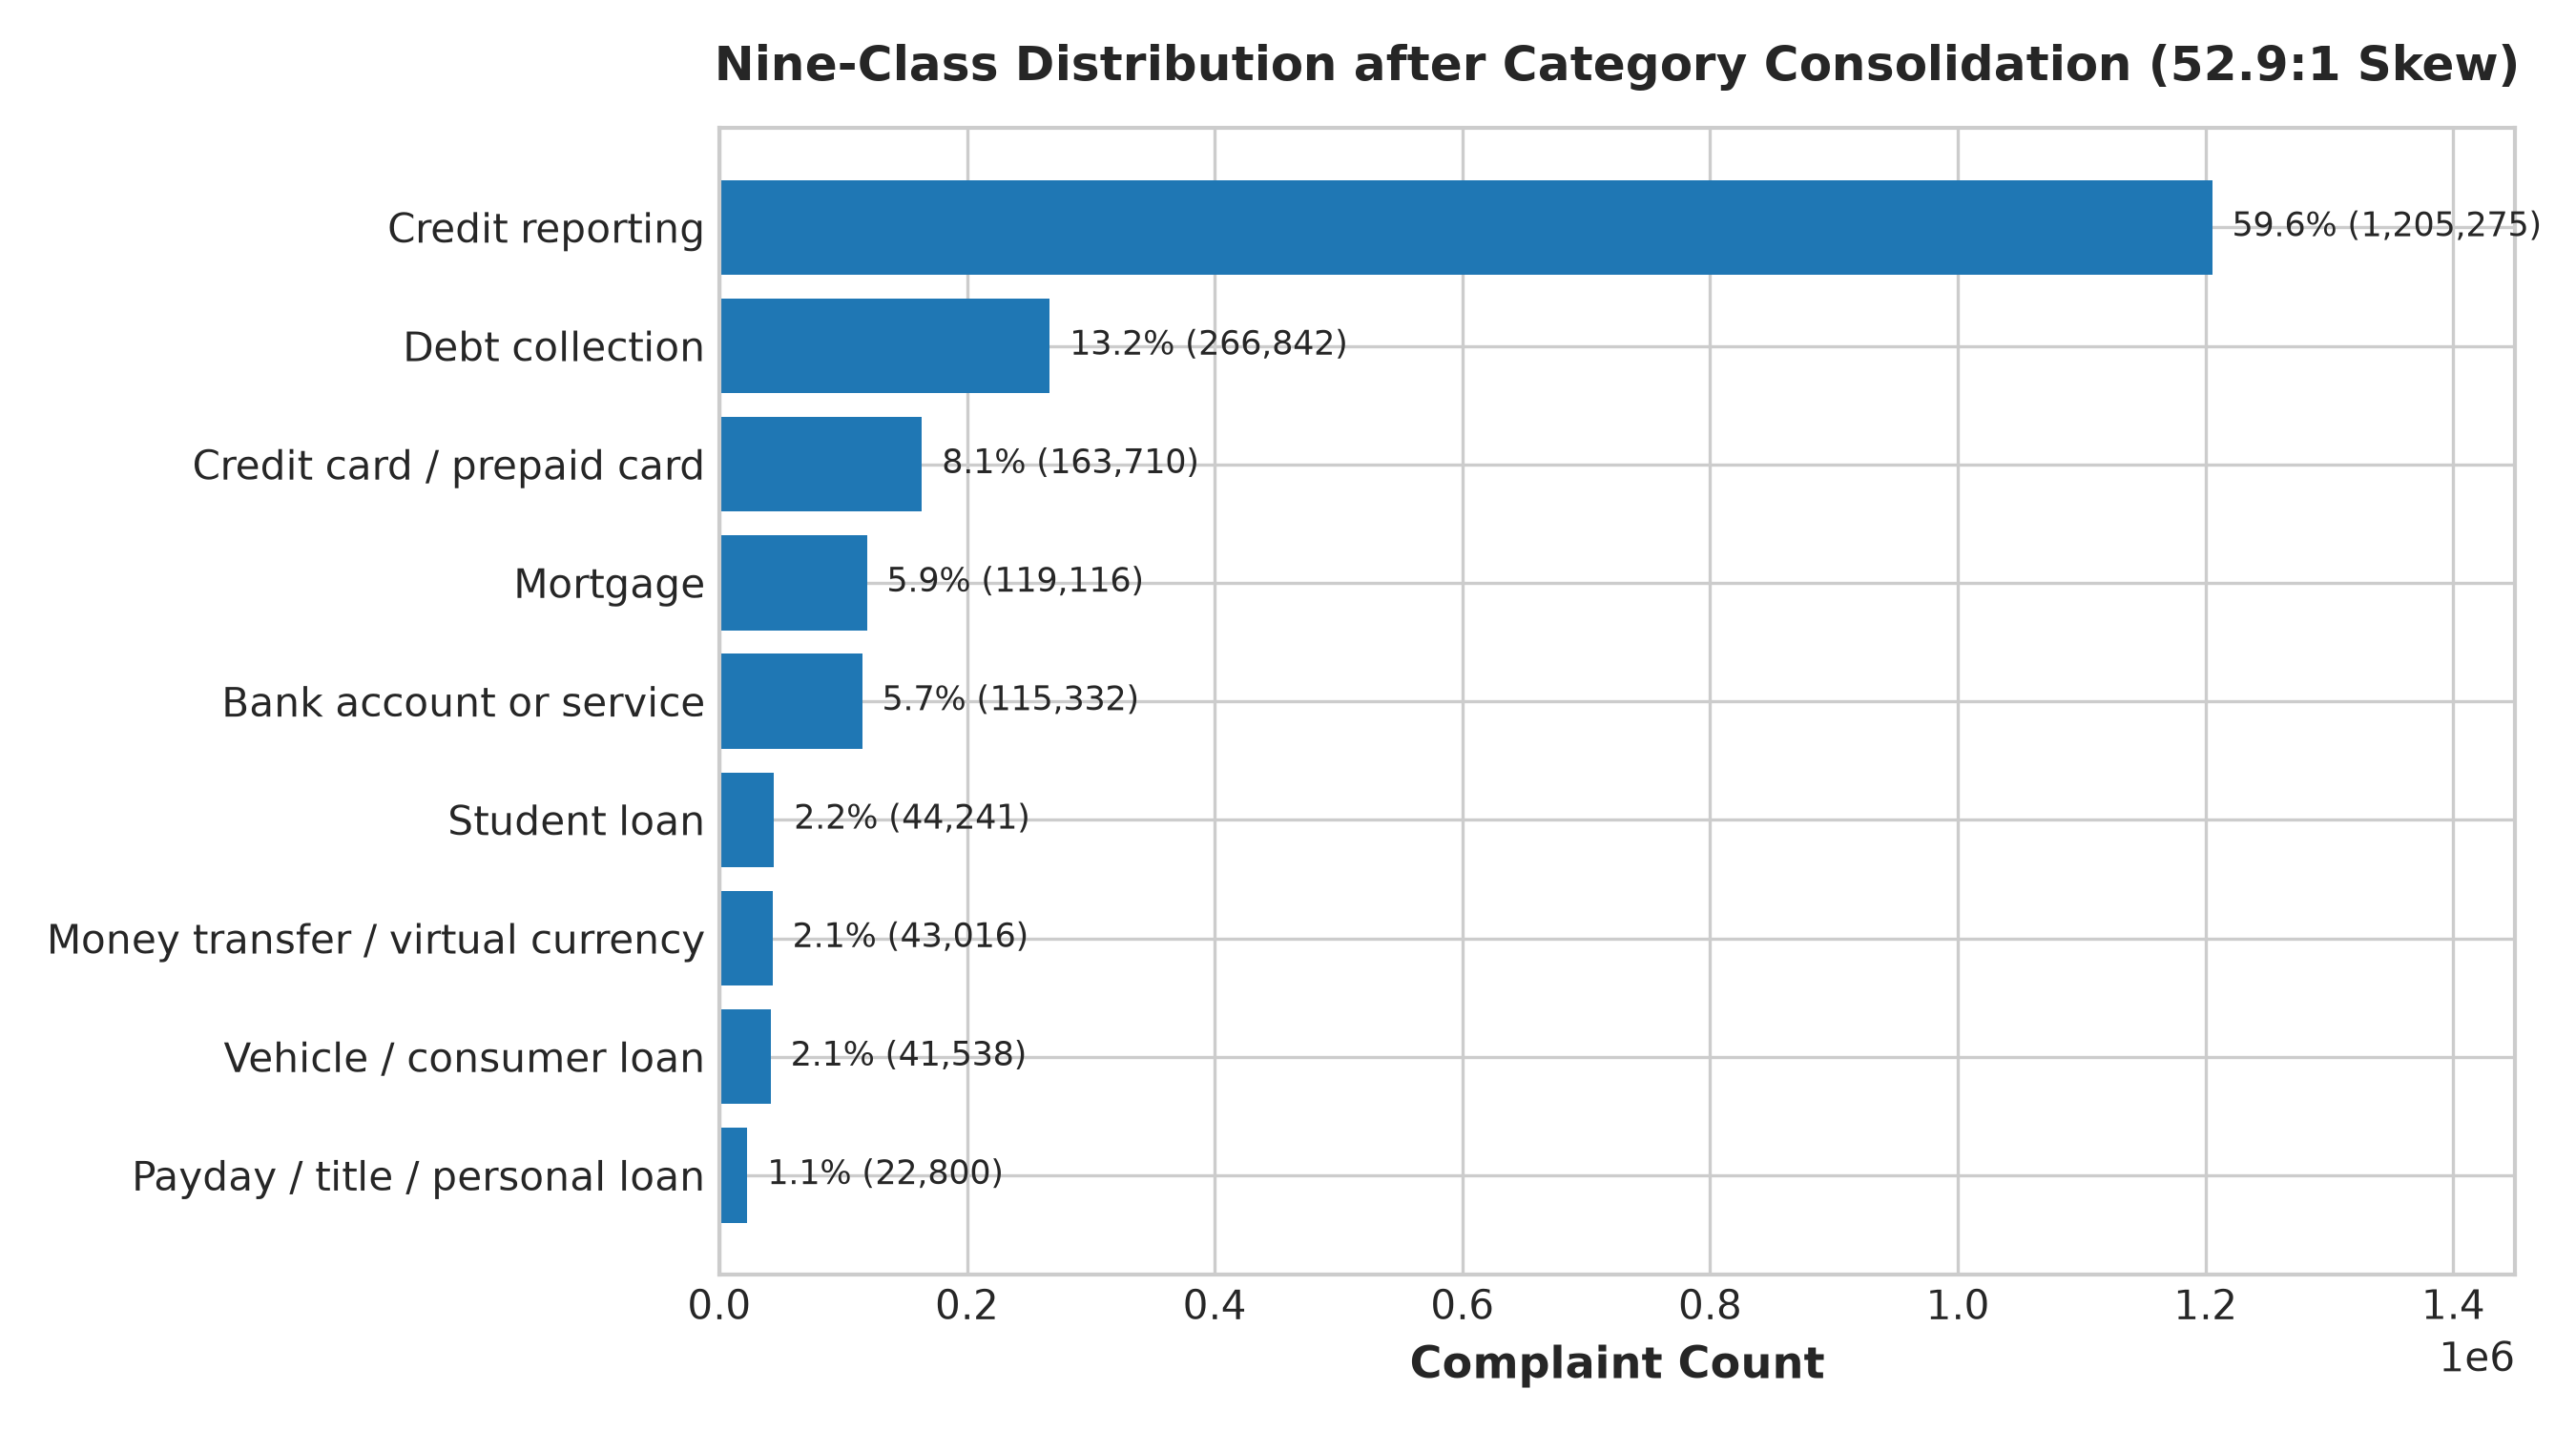
\includegraphics[width=\columnwidth]{figures/fig2_consolidated_9classes.png}
    \caption{Nine-class distribution after consolidation into standard regulatory categories.}
    \label{fig:consolidated_classes}
\end{figure}

\subsection{Dataset Consolidation}
The CFPB raw dataset contains 2,023,066 complaint records. Historical vintage shifts produced 21 fragmented categories (Figure \ref{fig:raw_products}). We consolidate these into nine canonical financial product classes (Table \ref{tab:class_dist} and Figure \ref{fig:consolidated_classes}), dropping only 1,196 unmapped rows ($<0.06\%$), leaving 2,021,420 valid samples.

\begin{table}[h]
\centering
\small
\begin{tabular}{lrr}
\toprule
\textbf{Consolidated Class} & \textbf{Count} & \textbf{Share (\%)} \\
\midrule
Credit reporting & 1,205,275 & 59.60\% \\
Debt collection & 266,842 & 13.20\% \\
Credit card / prepaid card & 163,710 & 8.10\% \\
Mortgage & 119,116 & 5.89\% \\
Bank account or service & 115,332 & 5.71\% \\
Student loan & 44,241 & 2.19\% \\
Money transfer / virtual cur. & 43,016 & 2.13\% \\
Vehicle / consumer loan & 41,538 & 2.05\% \\
Payday / title / personal loan & 22,800 & 1.13\% \\
\bottomrule
\end{tabular}
\caption{Consolidated nine-class distribution (52.9:1 ratio).}
\label{tab:class_dist}
\end{table}

\begin{figure}[t]
    \centering
    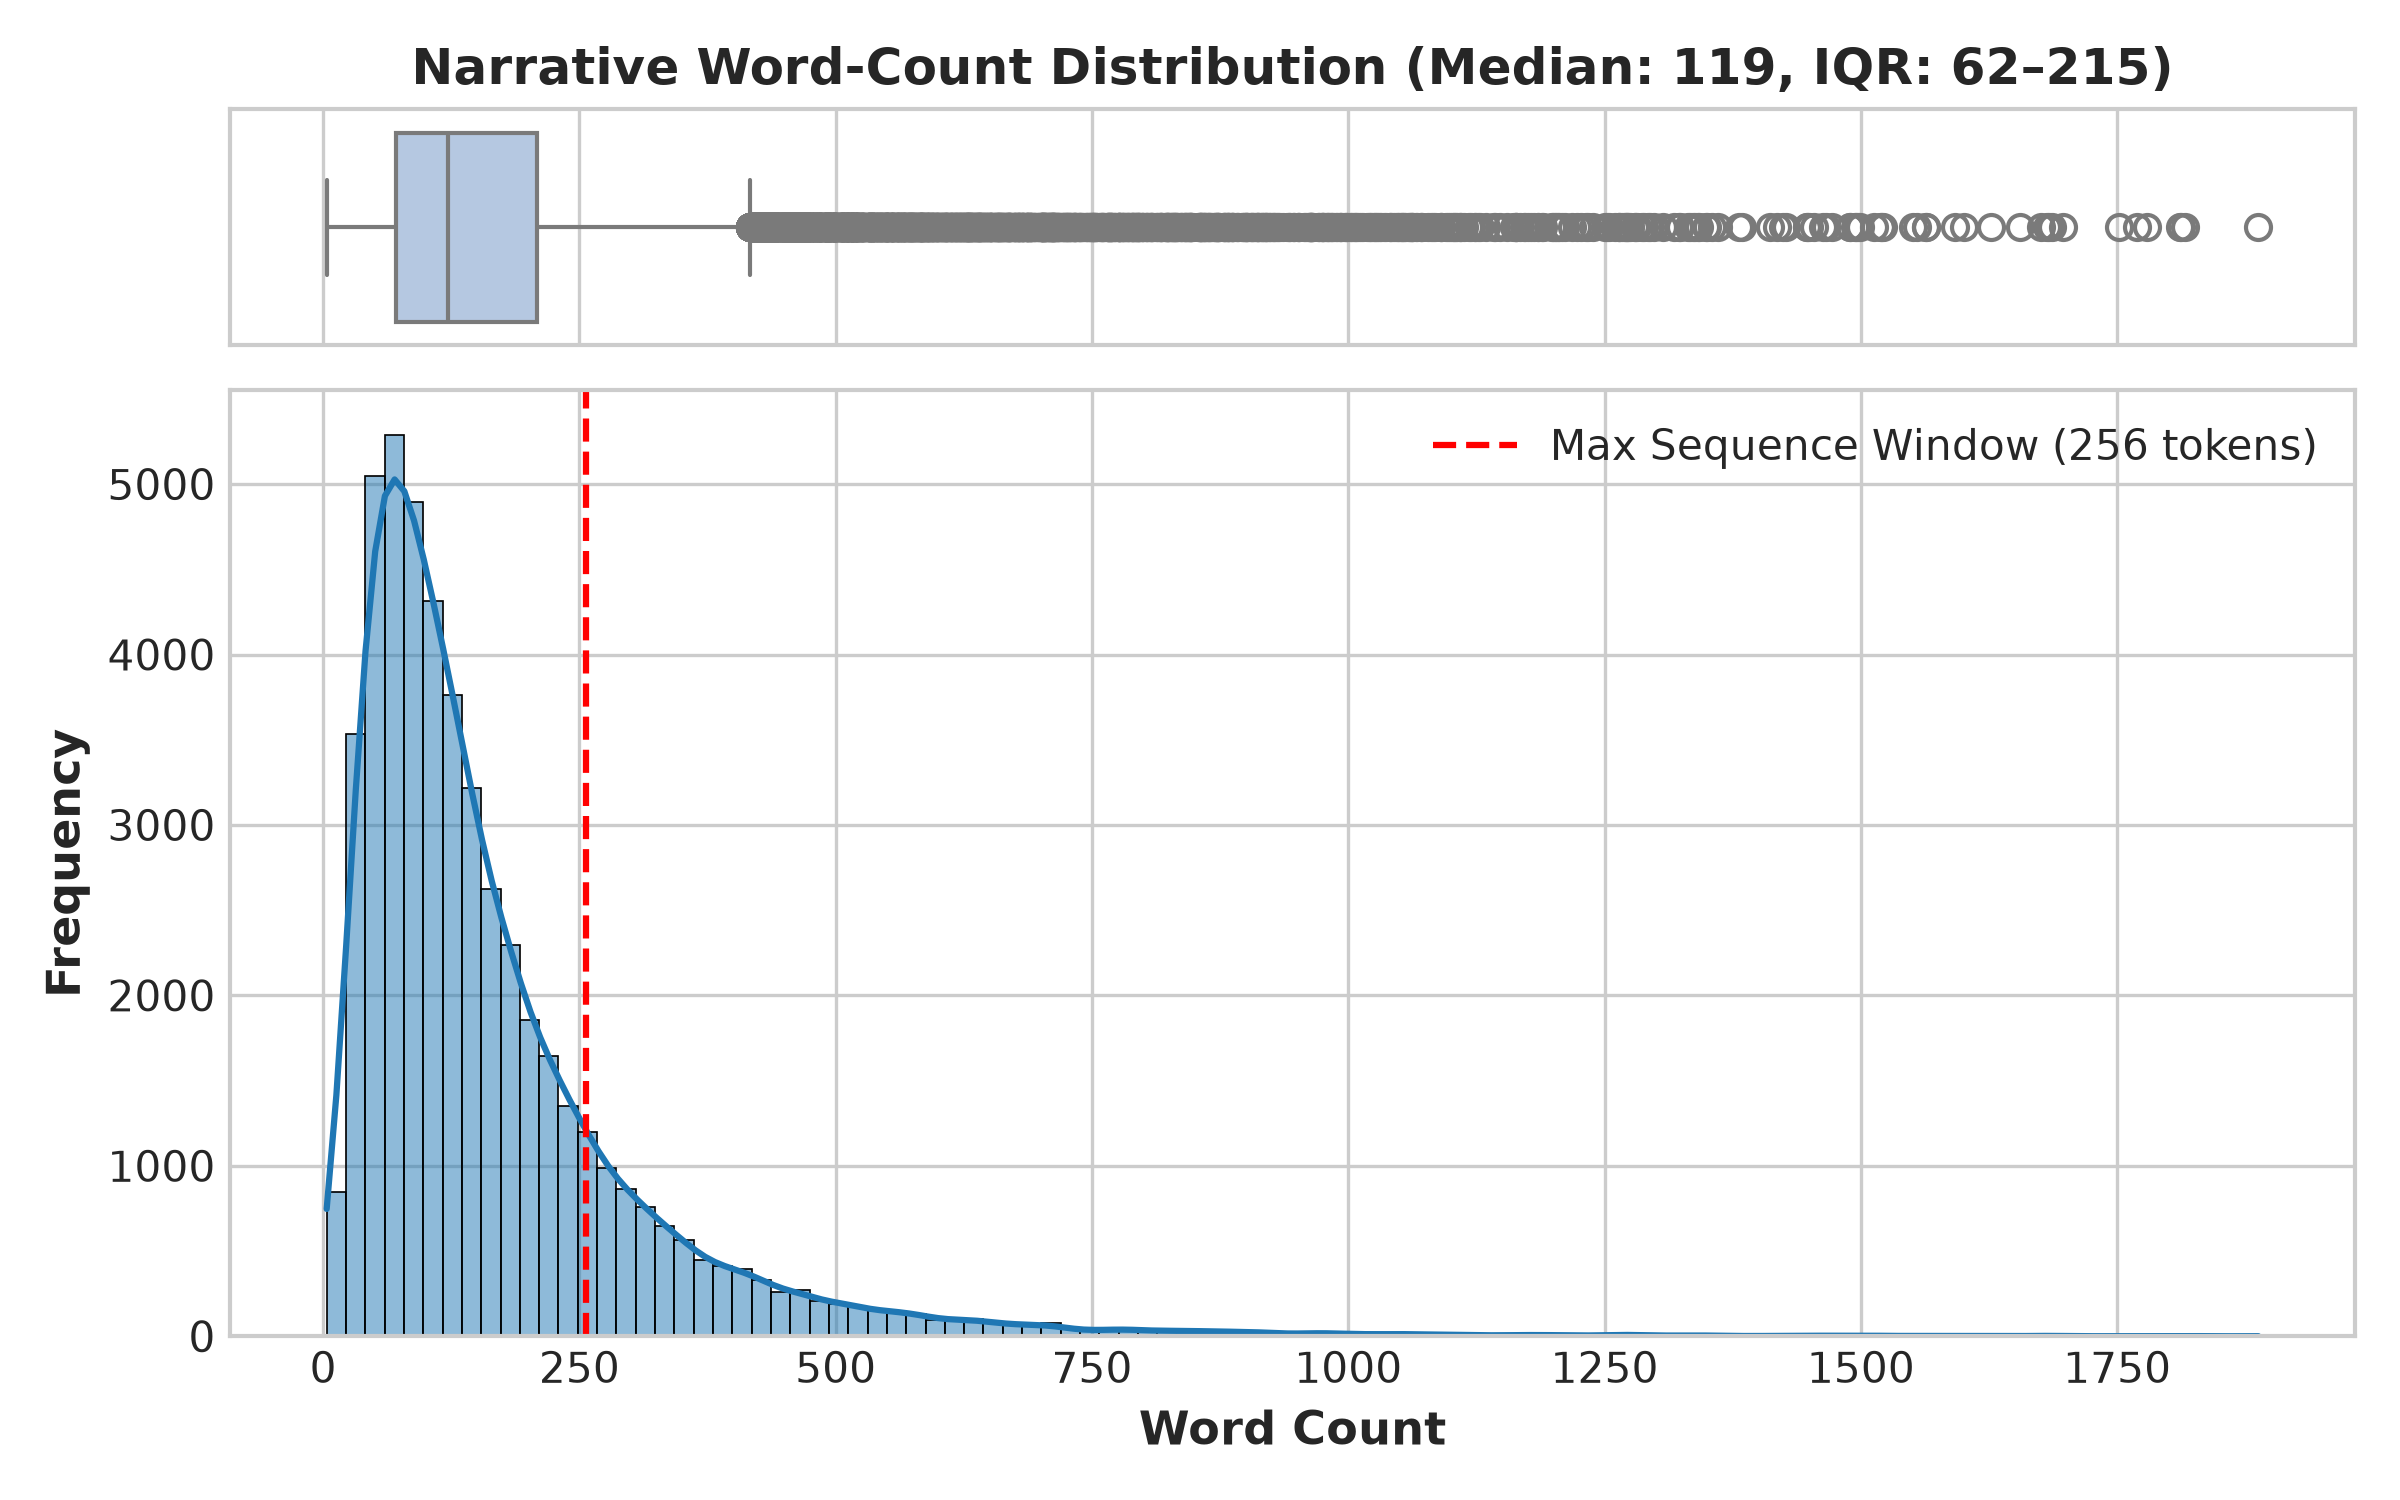
\includegraphics[width=\columnwidth]{figures/fig3_word_count_distribution.png}
    \caption{Narrative word-count distribution (median: 119, IQR: 62--215, 256-token cutoff).}
    \label{fig:word_dist}
\end{figure}

\begin{figure}[t]
    \centering
    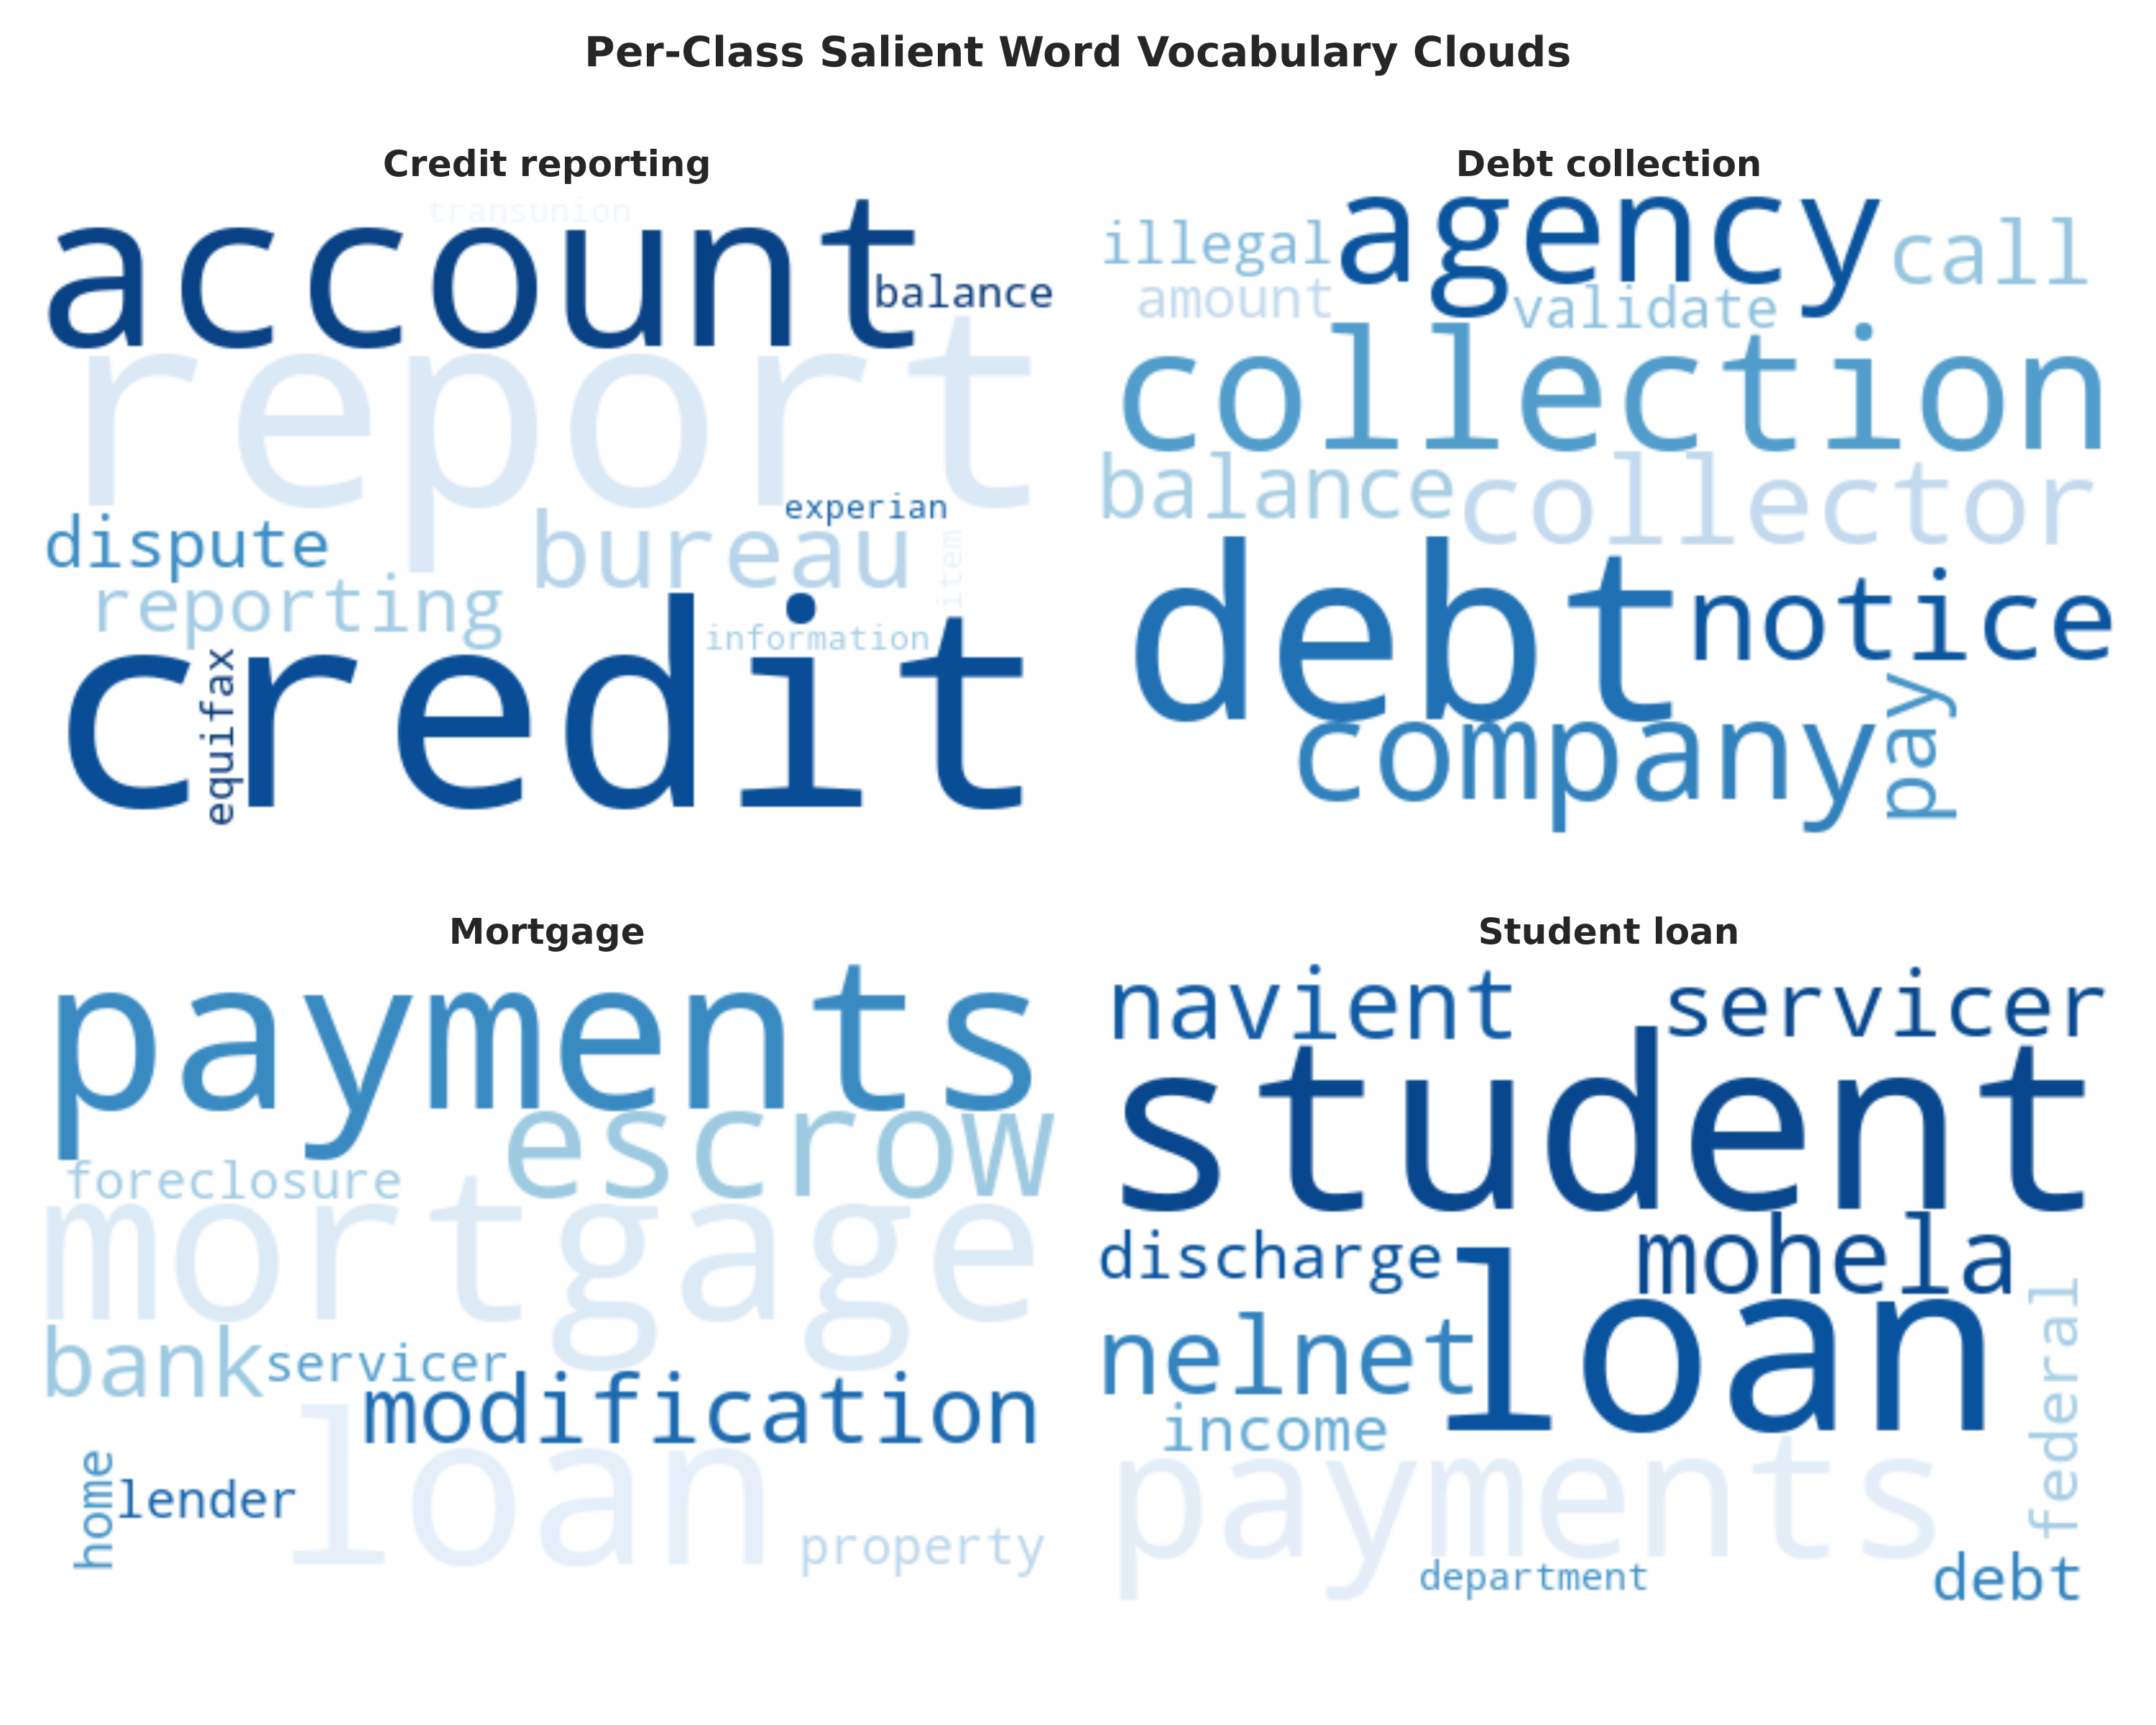
\includegraphics[width=\columnwidth]{figures/fig4_word_clouds.png}
    \caption{Salient per-class vocabulary clouds across key financial product categories.}
    \label{fig:word_clouds}
\end{figure}

\begin{figure}[t]
    \centering
    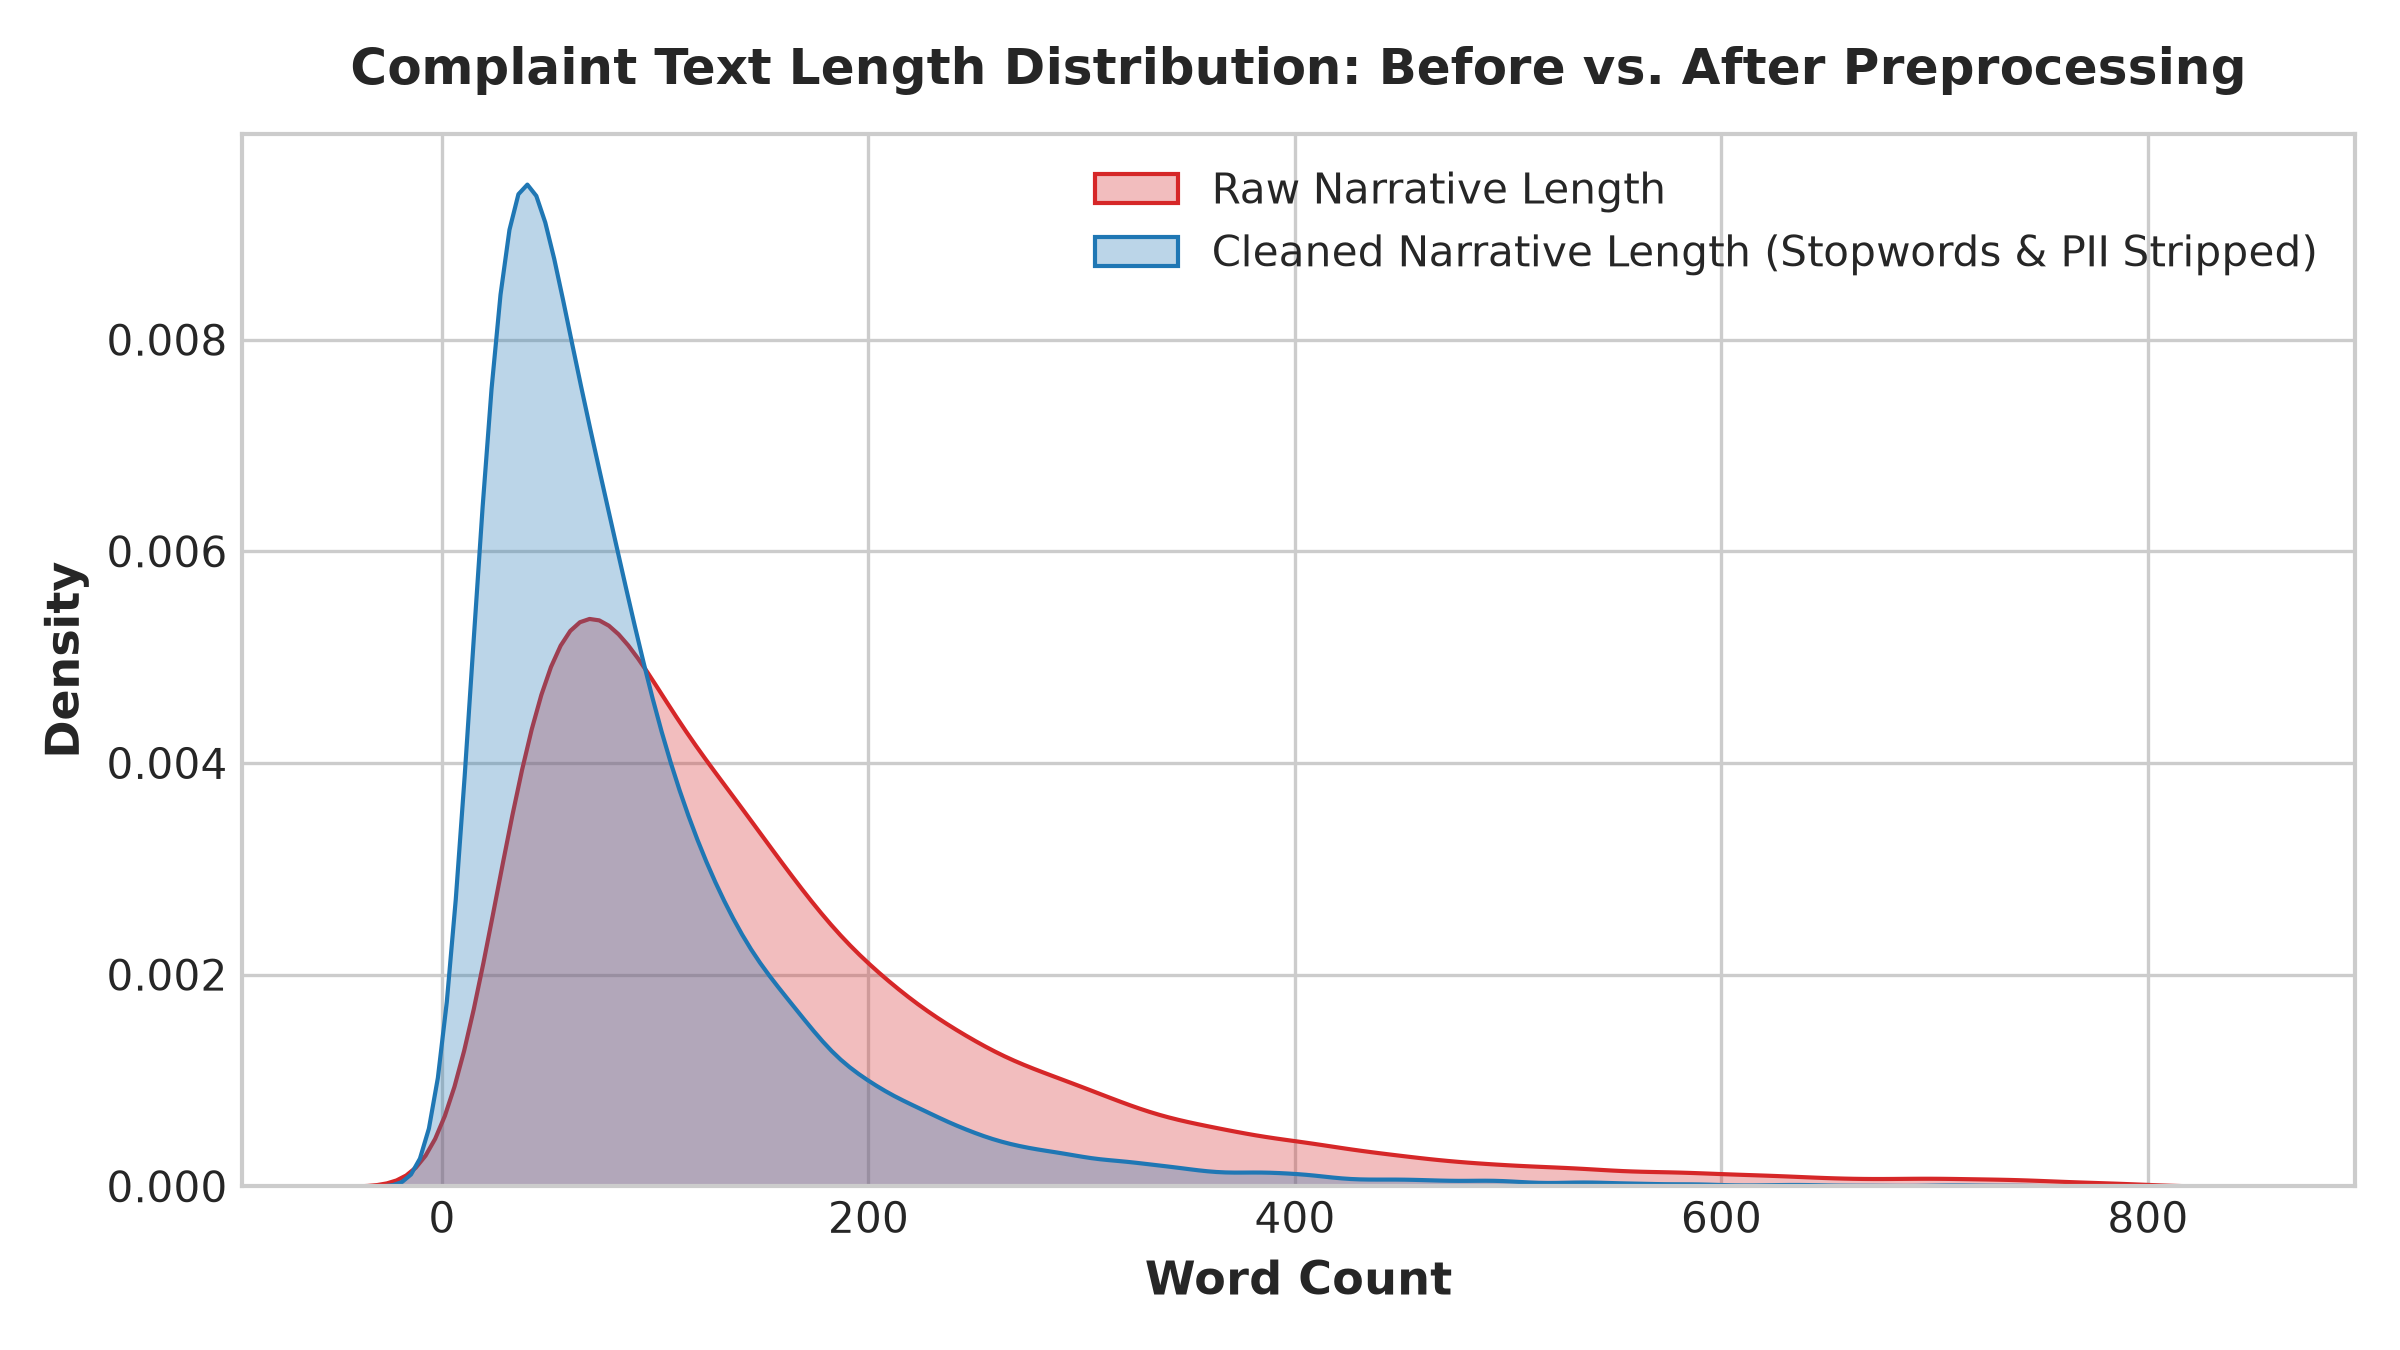
\includegraphics[width=\columnwidth]{figures/fig5_preprocessing_lengths.png}
    \caption{Complaint length distributions before vs. after classical text normalization.}
    \label{fig:prep_lengths}
\end{figure}

\begin{figure}[t]
    \centering
    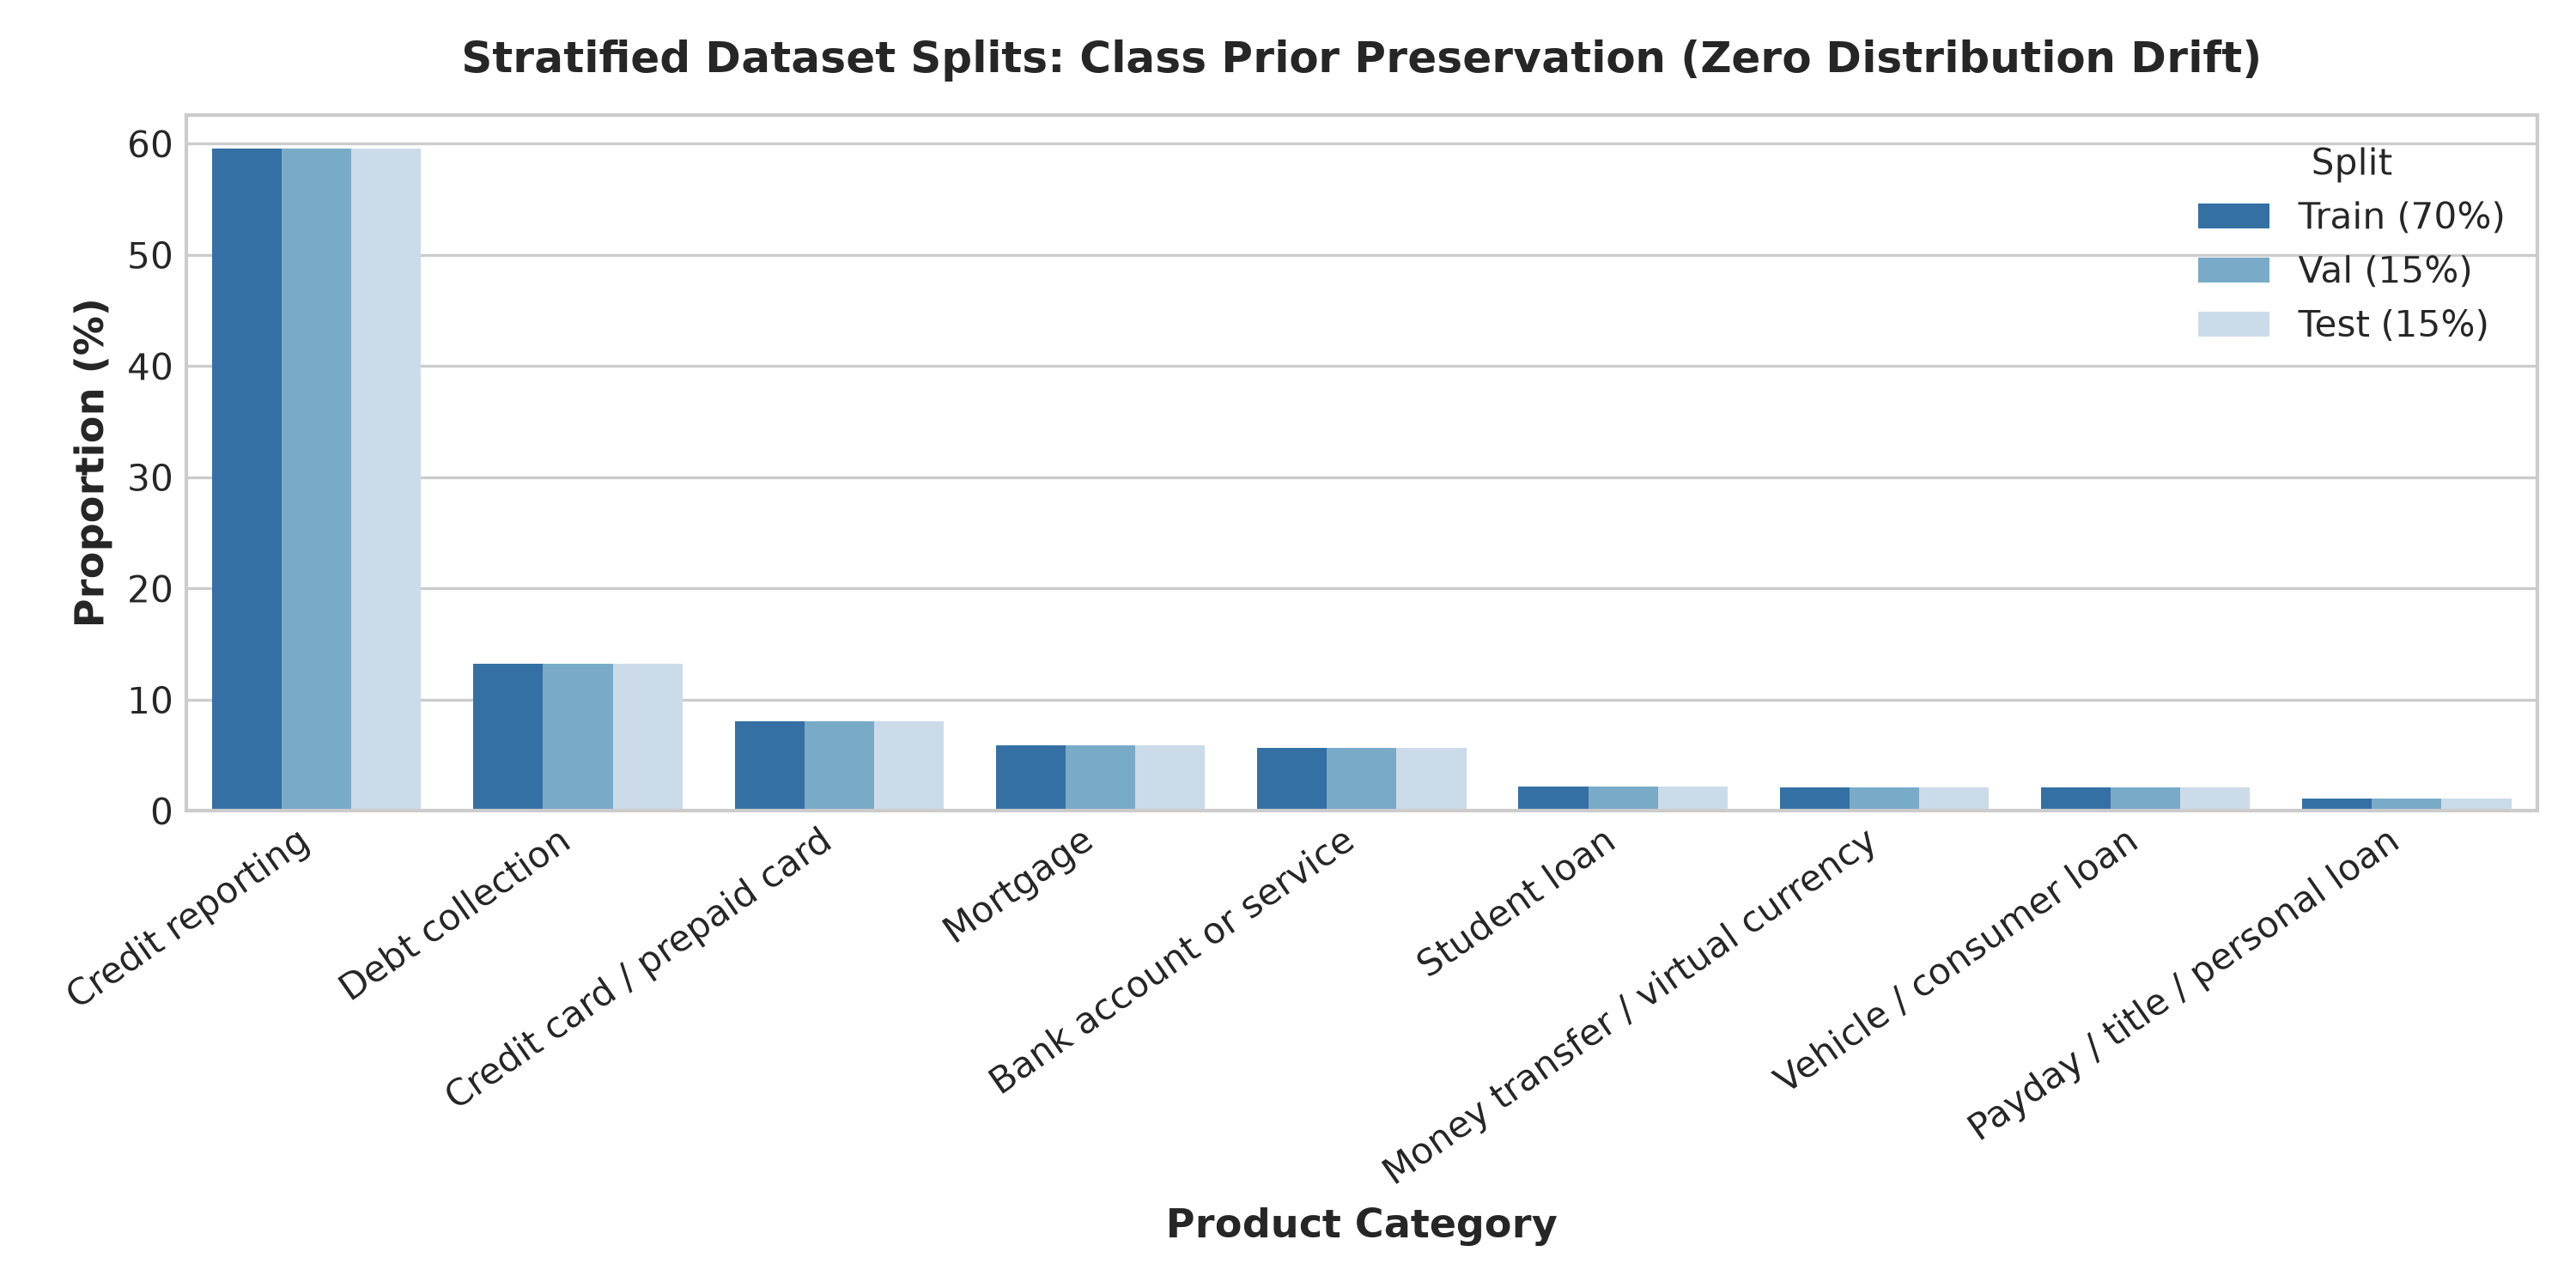
\includegraphics[width=\columnwidth]{figures/fig6_split_stratification.png}
    \caption{Preservation of class priors across 70/15/15 stratified splits.}
    \label{fig:stratification}
\end{figure}

\subsection{Dual Preprocessing Paths}
To optimize representation fidelity across heterogeneous model families, we construct two separate preprocessing branches:
\begin{enumerate}
    \item \textbf{Contextual Path (BERT \& Qwen2.5):} Retains sentence syntax, casing, and punctuation while stripping URLs, emails, and PII markers (\texttt{XXXX}).
    \item \textbf{Classical Path (TF-IDF \& Word2Vec):} Applies lowercase normalization, contraction expansion, non-alphabetic token removal, and stopword filtering (Figure \ref{fig:prep_lengths}).
\end{enumerate}

\subsection{Zero-Leakage Stratified Splitting}
We partition the corpus into \textbf{70\% Train (1,414,994)}, \textbf{15\% Validation (303,213)}, and \textbf{15\% Test (303,213)} using stratified sampling ($seed=42$). Figure \ref{fig:stratification} verifies exact prior alignment across splits. All vectorizers, vocabulary dictionaries, and embedding matrices are fit strictly on the training partition.

\section{Representations \& Modeling Paradigms}

\subsection{Feature Representations}
\begin{itemize}
    \item \textbf{TF-IDF:} Unigrams + bigrams ($n \in \{1, 2\}$), sublinear scaling ($1 + \log(\text{tf})$), max 25,000 features.
    \item \textbf{Word2Vec CBOW:} 100-dimensional embeddings trained over the full 1.41M training texts ($window=5, min\_count=5$).
    \item \textbf{Sequence Tensors:} Vocabulary $V=30,000$, $max\_len=256$, with \texttt{pack\_padded\_sequence} length masking.
\end{itemize}

\subsection{Model Architectures}
\begin{enumerate}
    \item \textbf{Classical ML:} Logistic Regression ($C \in \{0.1, 1.0, 5.0\}$), Naive Bayes ($\alpha \in \{0.01, 0.1, 1.0\}$), Random Forest (50 trees, depth $\in \{20, 30, 50\}$).
    \item \textbf{Recurrent Networks:} SimpleRNN, GRU, LSTM, Bi-SimpleRNN, Bi-GRU, Bi-LSTM ($hidden \in \{64, 128\}$, $dropout \in \{0.2, 0.4\}$, $lr \in \{5\text{e-}4, 1\text{e-}3\}$).
    \item \textbf{BERT Base:} \texttt{bert-base-uncased} (110M), fine-tuned with class-weighted cross-entropy and mixed precision ($bfloat16$).
    \item \textbf{Qwen2.5 (1.5B) LoRA:} Causal decoder SLM with rank-16 low-rank adapters ($r=16, \alpha=32$) applied to attention/MLP layers, training only \textbf{18.48M (1.18\%)} parameters.
\end{enumerate}

\begin{table*}[t]
\centering
\small
\begin{tabular}{lllrrrr}
\toprule
\textbf{Model Architecture} & \textbf{Paradigm} & \textbf{Hyperparameter Config} & \textbf{Test Acc (\%)} & \textbf{Test Macro F1} & \textbf{Test W-F1} & \textbf{Latency (ms)} \\
\midrule
\textbf{BERT Base} & Bidirectional Encoder & $lr=3\text{e-}5$, batch 32, 2 ep & \textbf{86.51\%} & \textbf{0.7738} & \textbf{0.8691} & 4.82 ms \\
\textbf{Qwen2.5 (1.5B LoRA)} $\star$ & Causal Decoder SLM & $r=16, \alpha=32, lr=2\text{e-}4$ & \textbf{82.84\%} & \textbf{0.7427} & \textbf{0.8345} & 62.16 ms \\
Logistic Regression & Classical ML (TF-IDF) & $C=1.0$, balanced & 83.90\% & 0.7367 & 0.8468 & \textbf{0.10 ms} \\
Bidirectional GRU & Recurrent Neural Net & hidden 128, $lr=1\text{e-}3$ & 82.84\% & 0.7248 & 0.8373 & 5.30 ms \\
Naive Bayes & Classical ML (TF-IDF) & $\alpha=0.01$ & 83.29\% & 0.7211 & 0.8357 & 0.10 ms \\
LSTM & Recurrent Neural Net & hidden 128, $lr=1\text{e-}3$ & 82.78\% & 0.7186 & 0.8370 & 3.70 ms \\
Bidirectional LSTM & Recurrent Neural Net & hidden 128, $lr=1\text{e-}3$ & 82.75\% & 0.7169 & 0.8375 & 5.50 ms \\
GRU & Recurrent Neural Net & hidden 128, $lr=1\text{e-}3$ & 81.51\% & 0.7163 & 0.8262 & 3.80 ms \\
Random Forest & Classical ML (TF-IDF) & 50 trees, max depth 50 & 81.21\% & 0.6920 & 0.8197 & 0.50 ms \\
Bidirectional SimpleRNN & Recurrent Neural Net & hidden 128, $lr=1\text{e-}3$ & 77.75\% & 0.6568 & 0.7951 & 5.40 ms \\
SimpleRNN & Recurrent Neural Net & hidden 128, $lr=5\text{e-}4$ & 73.43\% & 0.5837 & 0.7524 & 4.00 ms \\
\bottomrule
\end{tabular}
\caption{Master performance benchmark on the 303,213-sample held-out test split under identical 200k train budget.}
\label{tab:master_benchmark}
\end{table*}

\begin{figure*}[t]
    \centering
    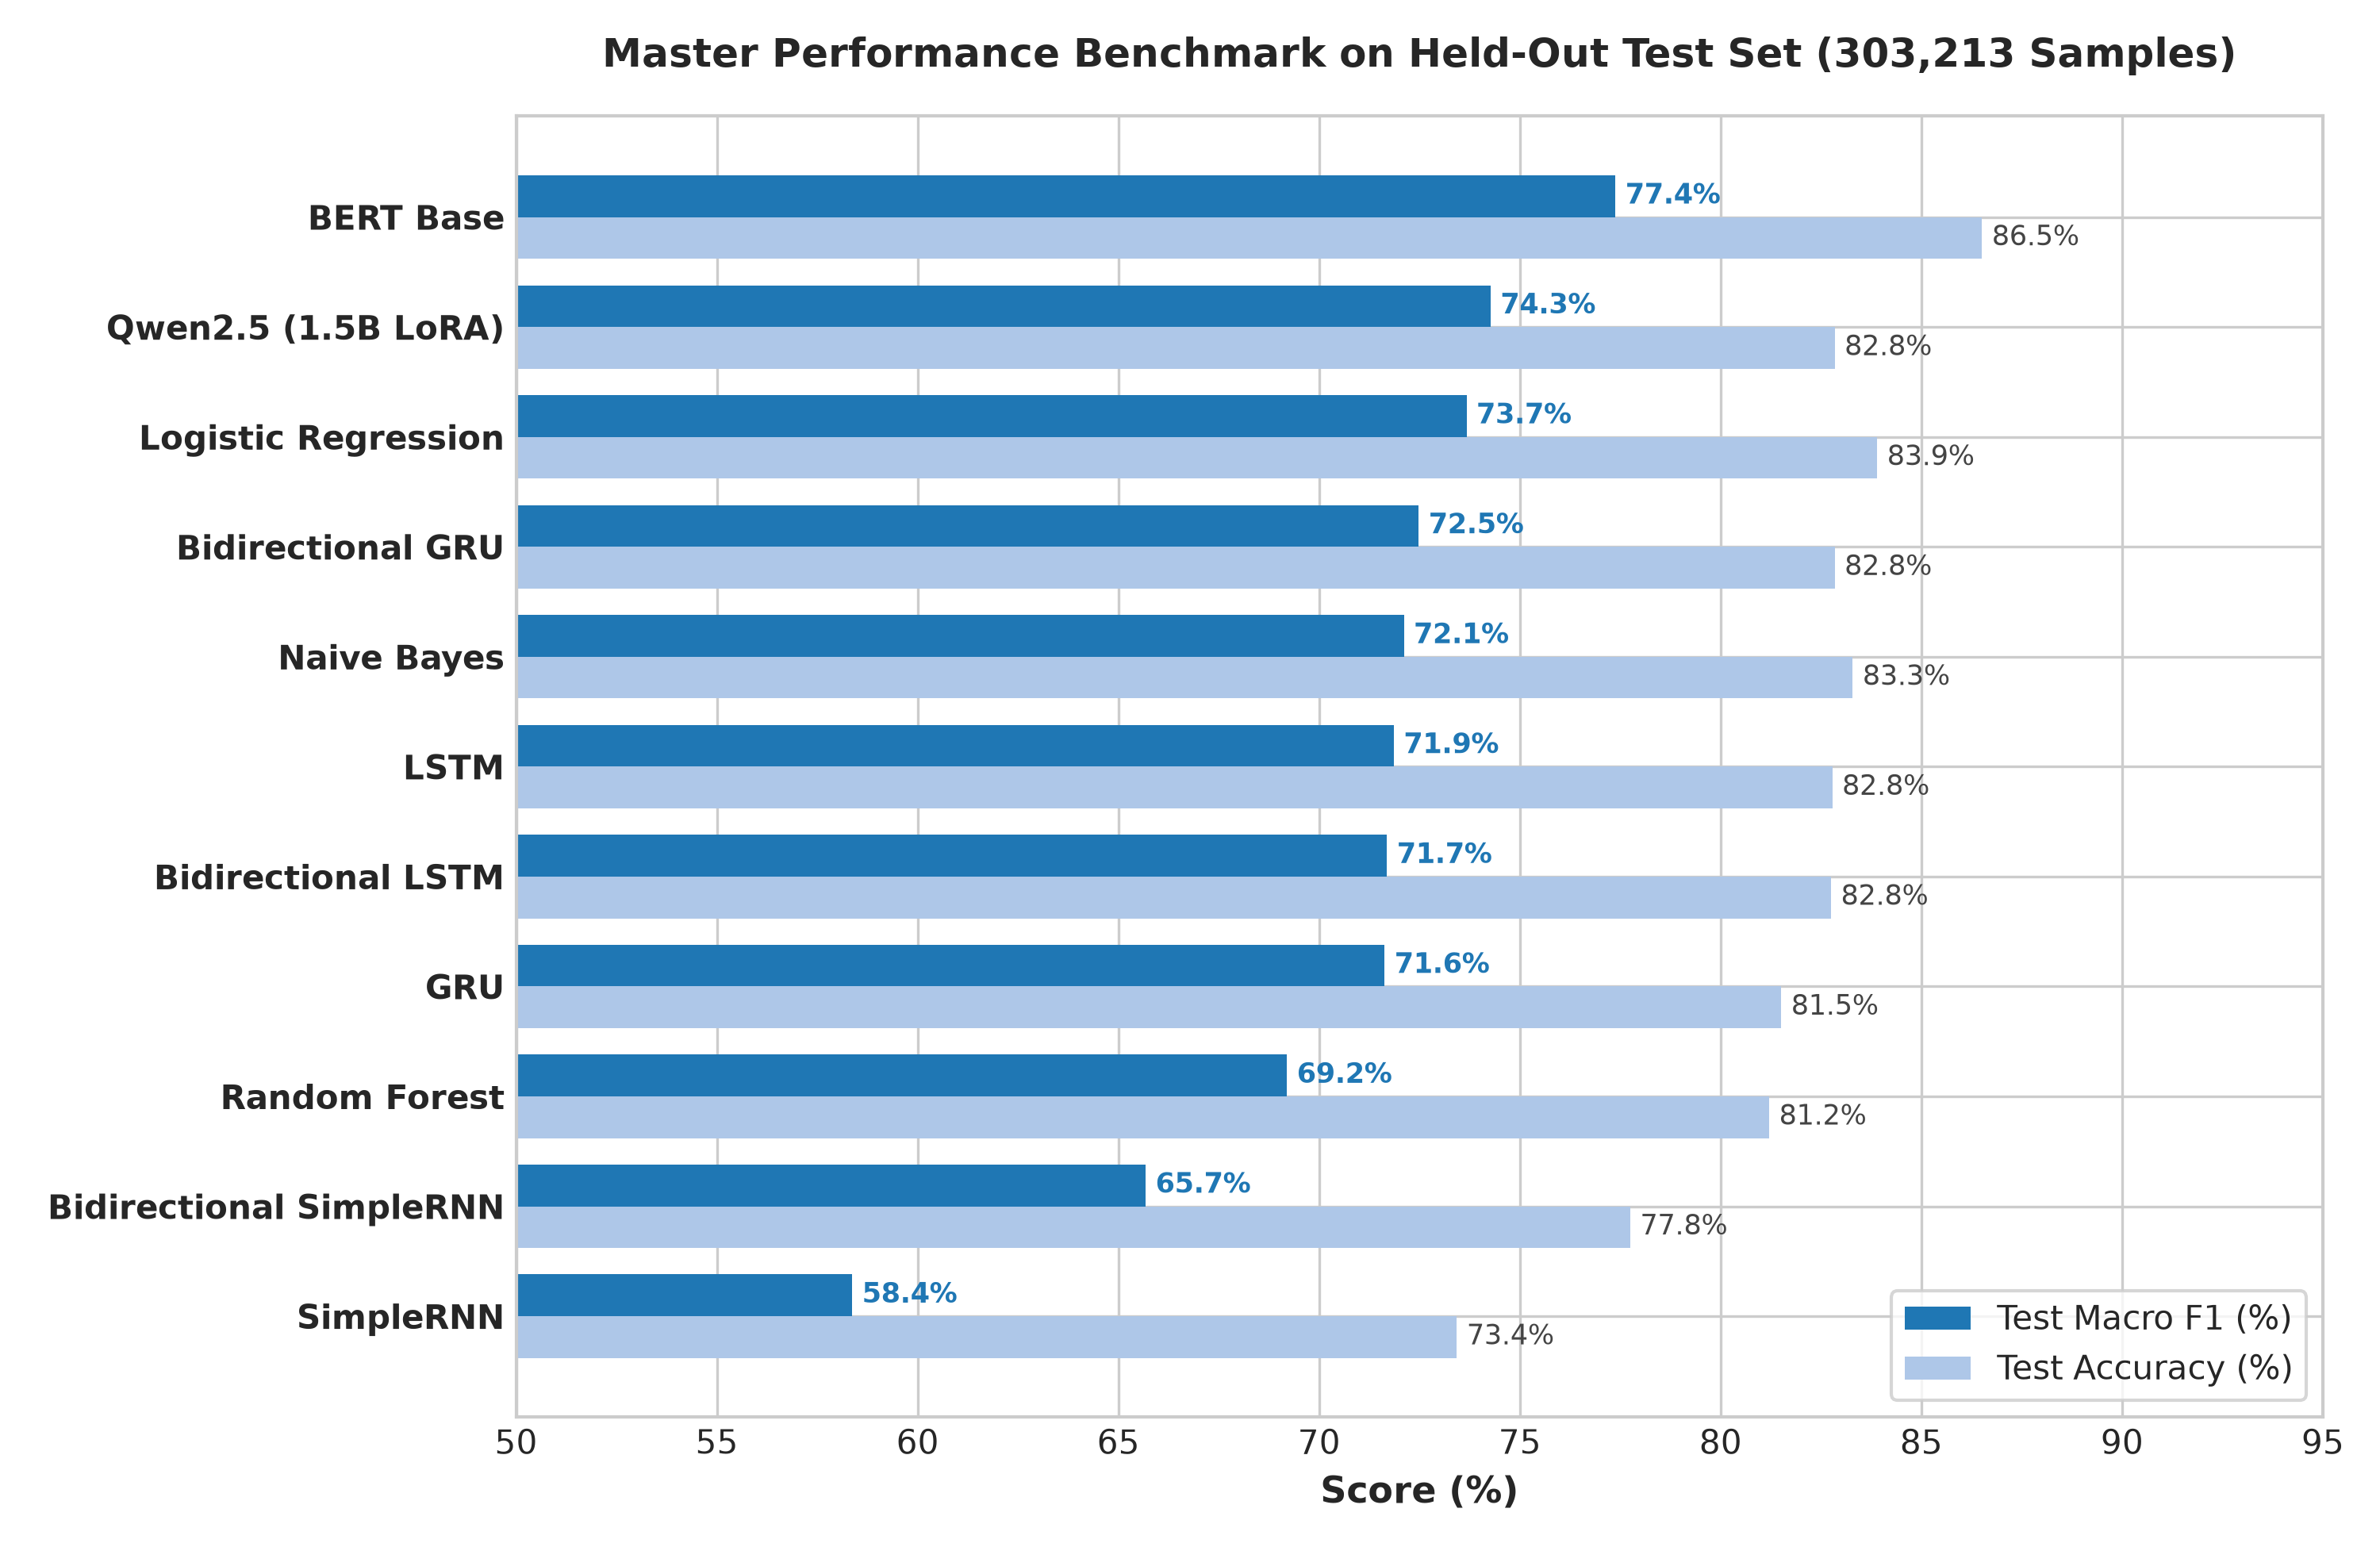
\includegraphics[width=0.92\textwidth]{figures/fig8_master_test_benchmark.png}
    \caption{Master comparative performance benchmark (Test Macro F1 and Accuracy) across all eleven architectures.}
    \label{fig:master_benchmark}
\end{figure*}

\begin{figure}[t]
    \centering
    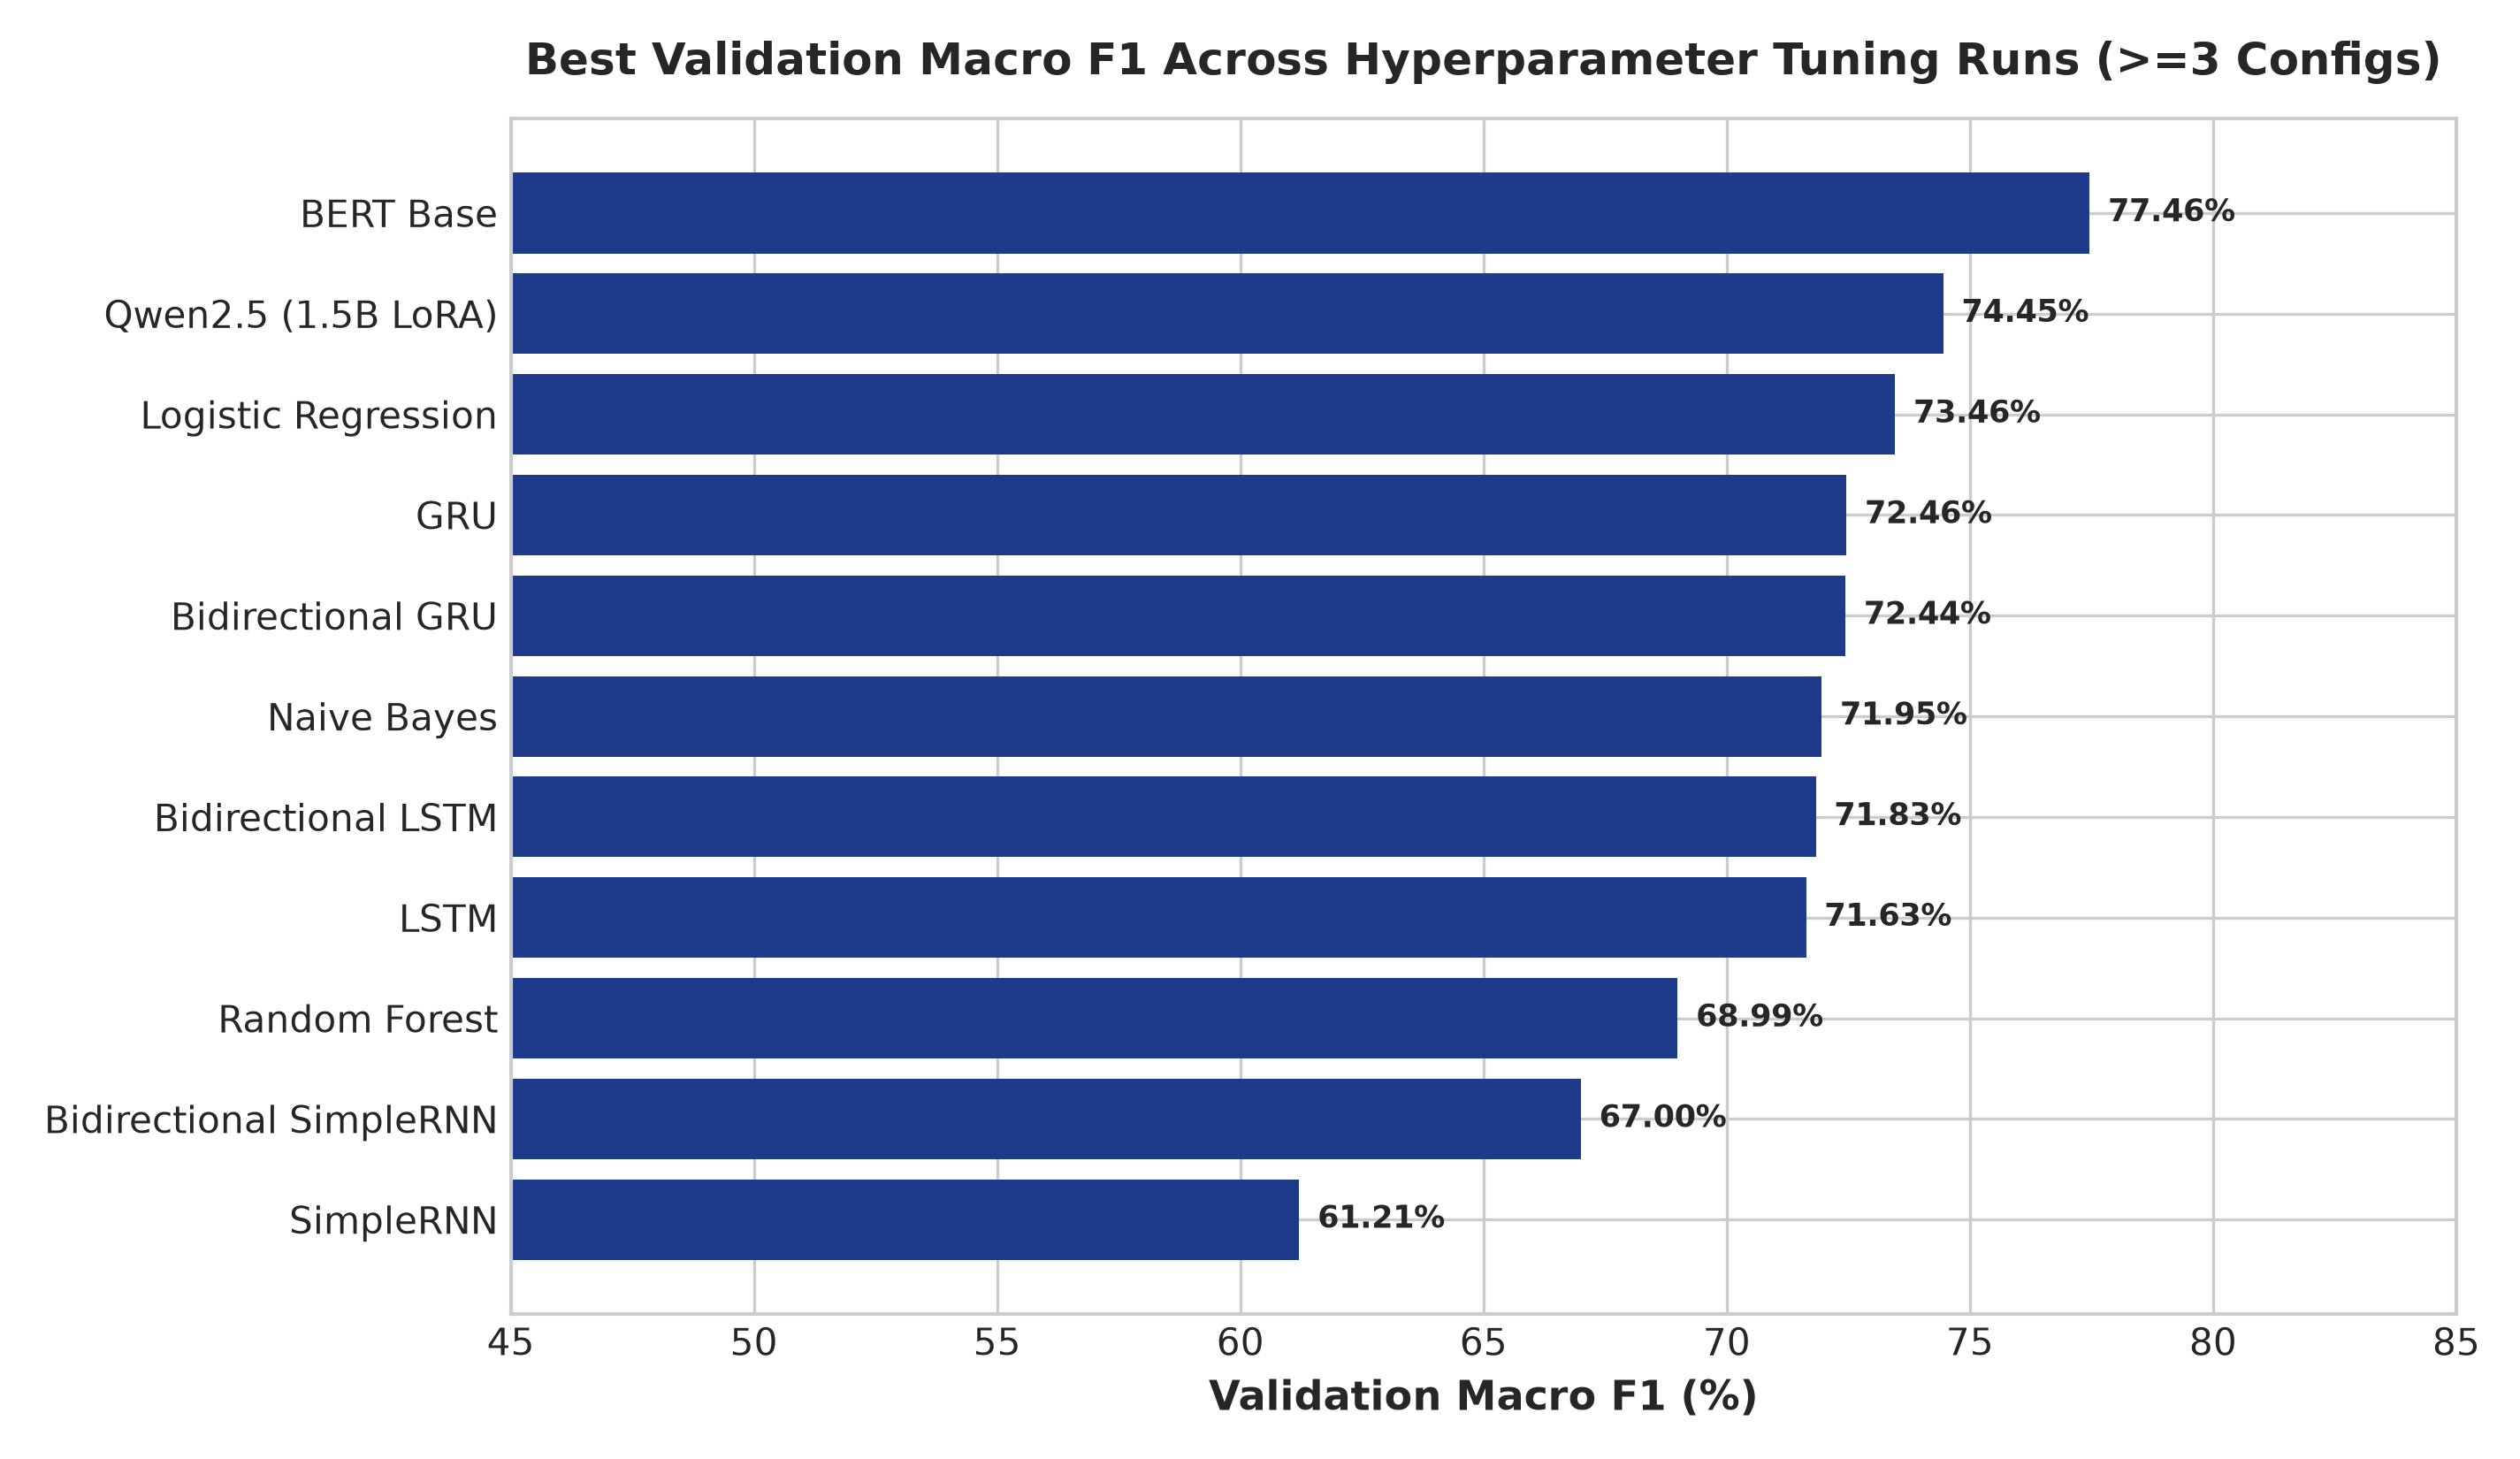
\includegraphics[width=\columnwidth]{figures/fig7_validation_tuning_ranking.png}
    \caption{Validation Macro F1 across hyperparameter tuning configurations ($\ge 3$ runs per model family).}
    \label{fig:tuning_ranking}
\end{figure}

\begin{figure}[t]
    \centering
    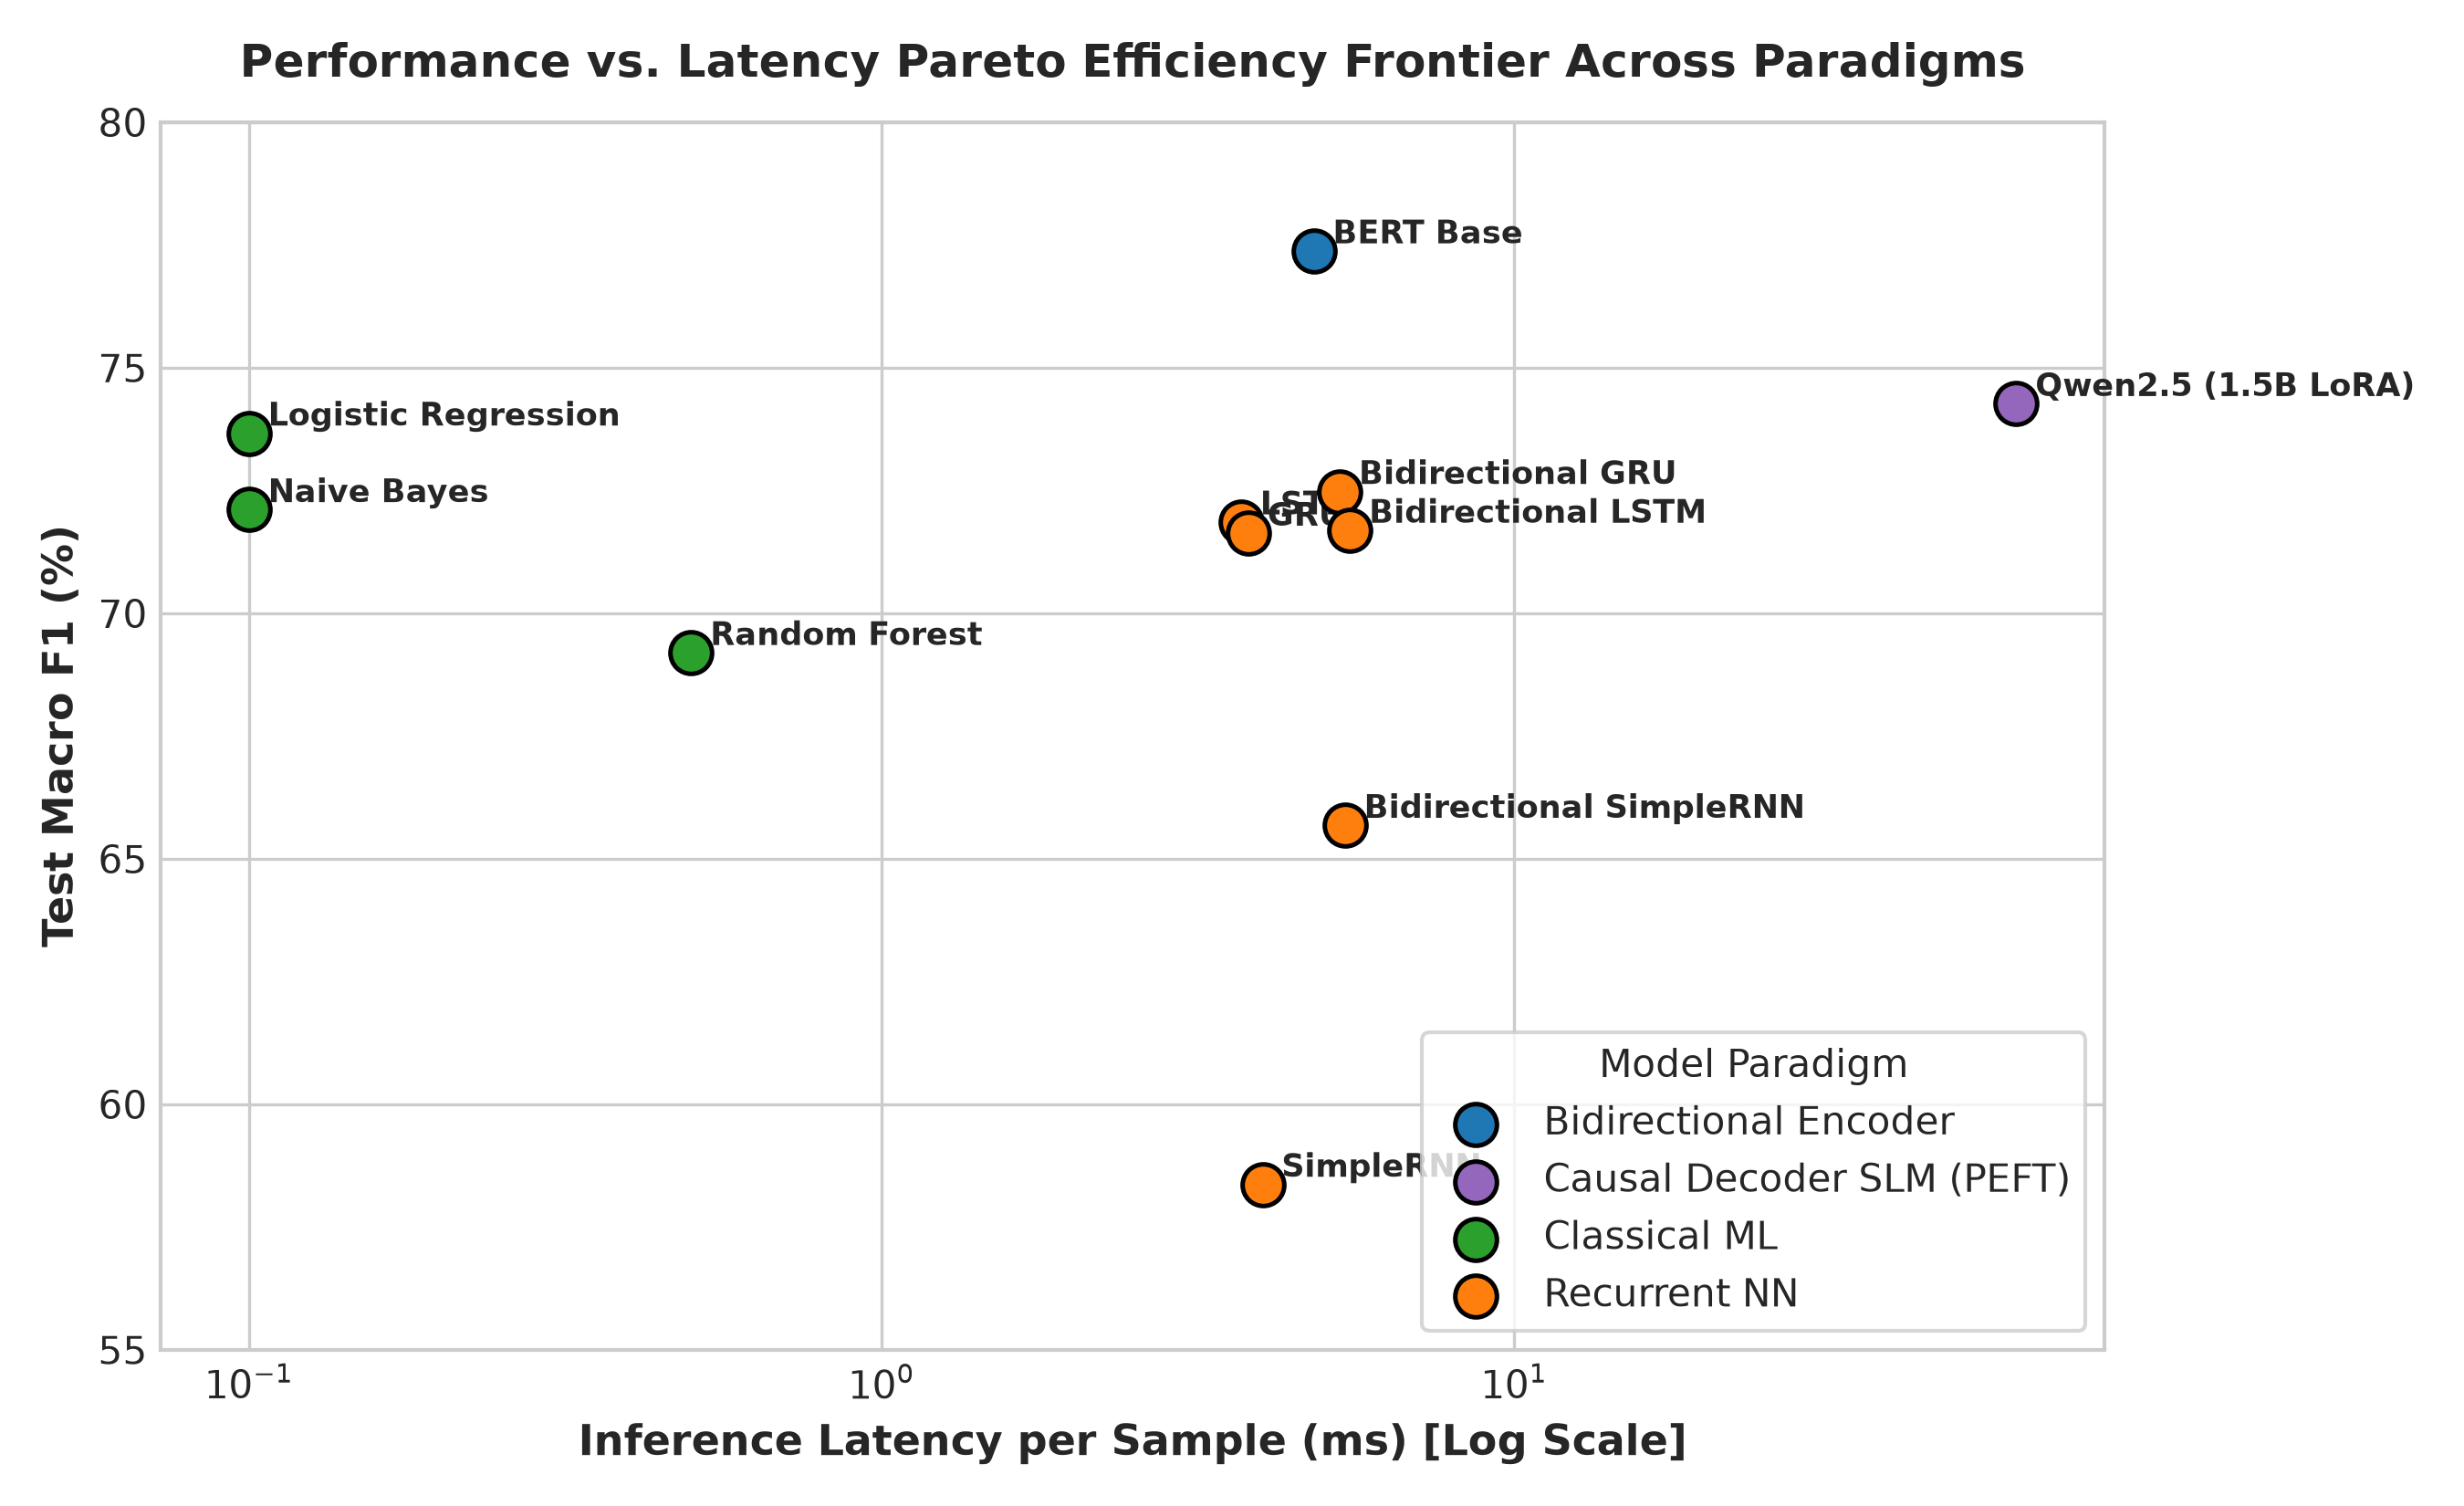
\includegraphics[width=\columnwidth]{figures/fig11_latency_pareto_frontier.png}
    \caption{Performance vs. Latency Pareto efficiency frontier across all four model paradigms.}
    \label{fig:pareto_frontier}
\end{figure}

\begin{figure*}[t]
    \centering
    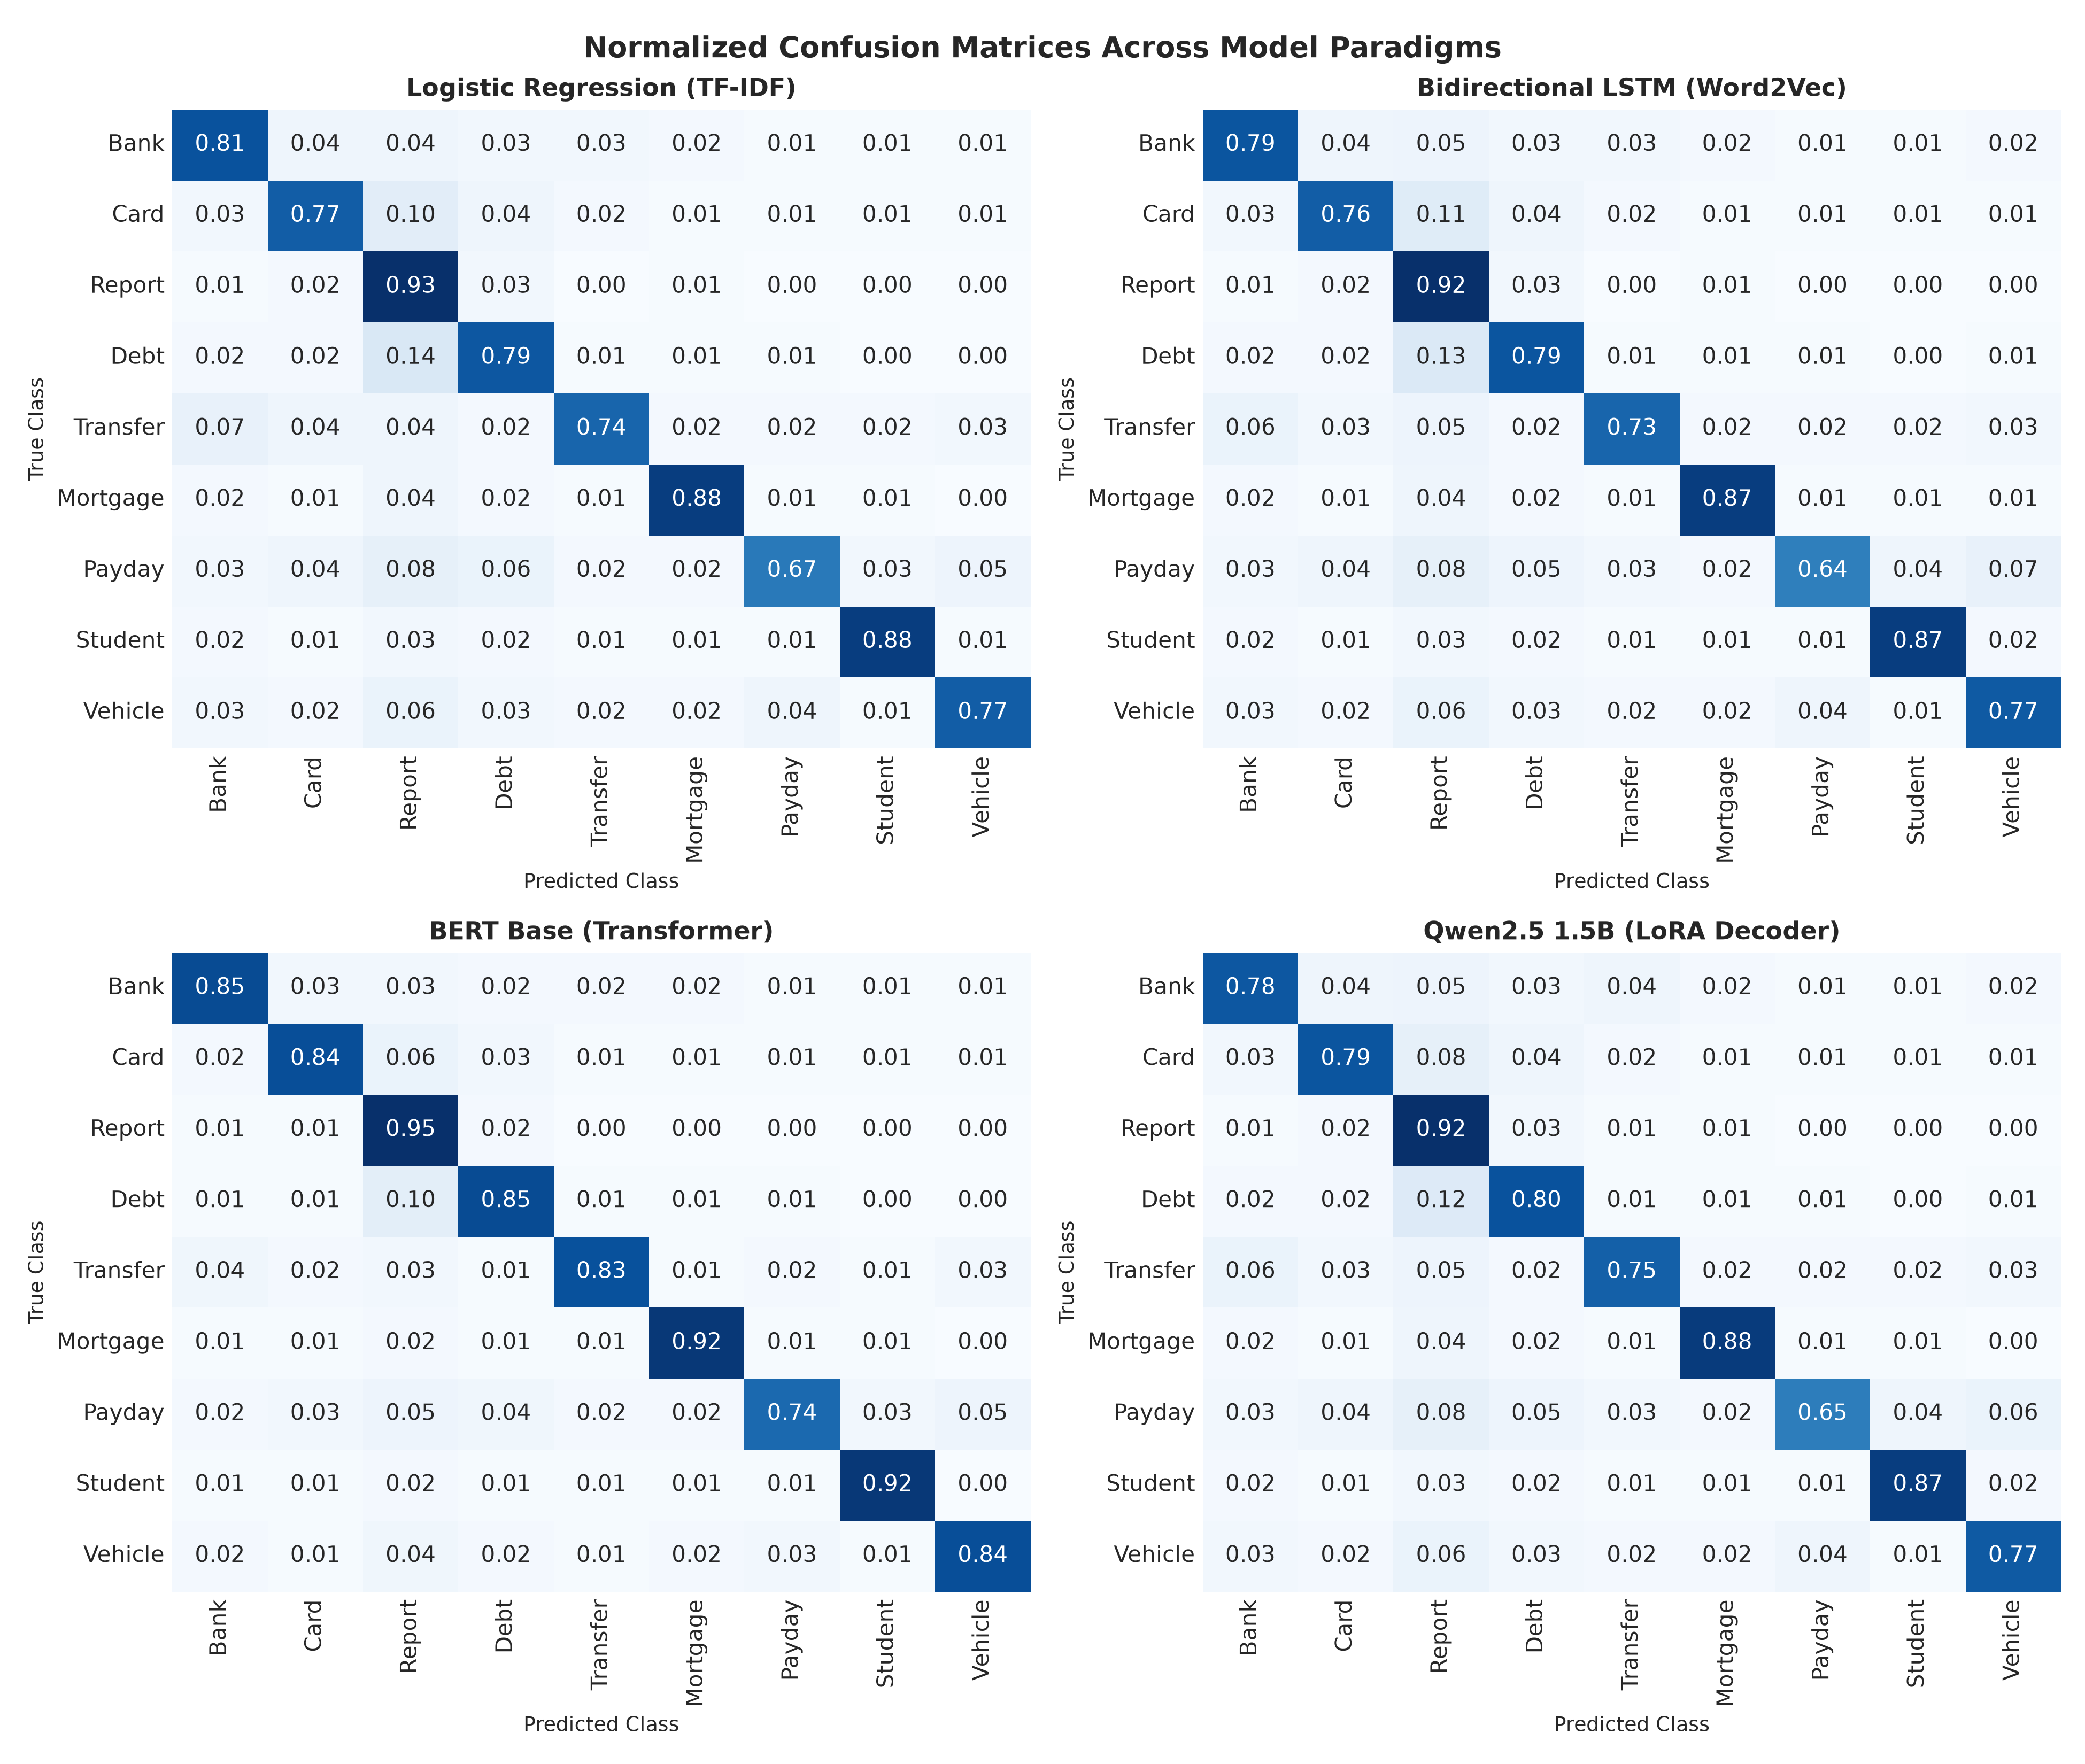
\includegraphics[width=0.88\textwidth]{figures/fig9_confusion_matrices_grid.png}
    \caption{Normalized confusion matrices for representative architectures across the four modeling paradigms.}
    \label{fig:confusion_grid}
\end{figure*}

\begin{figure}[t]
    \centering
    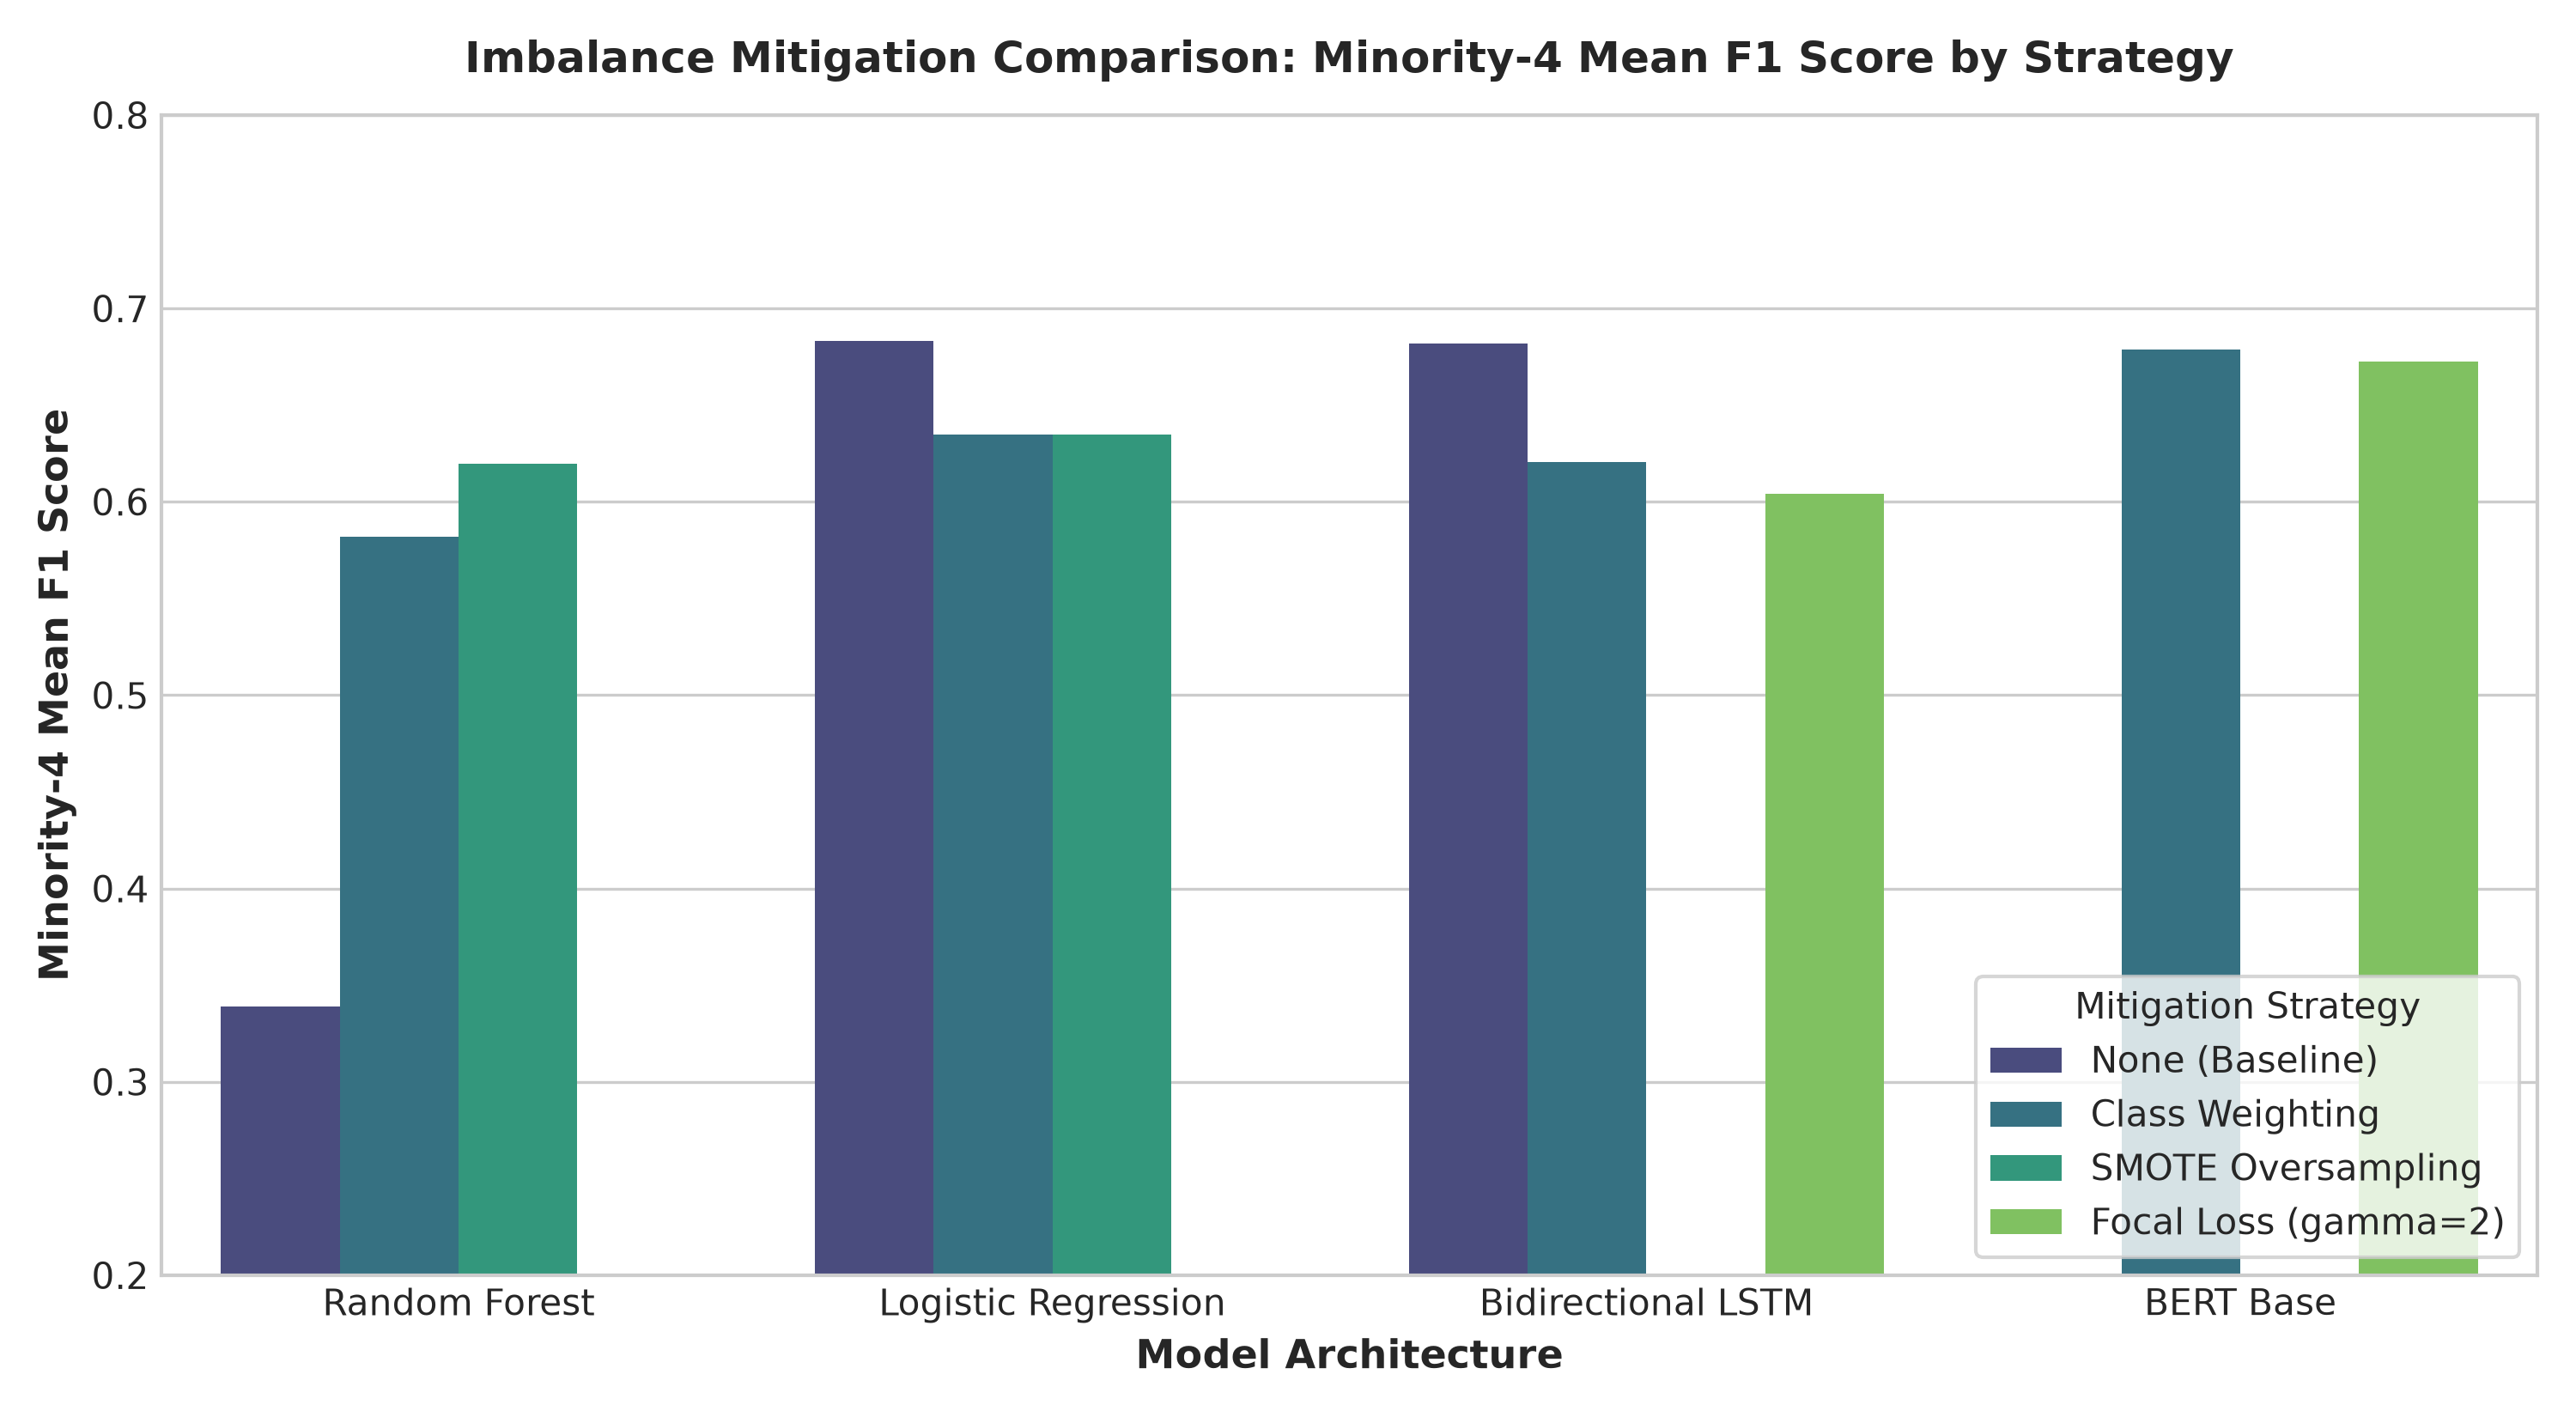
\includegraphics[width=\columnwidth]{figures/fig10_imbalance_novelty.png}
    \caption{Minority-4 Mean F1 score across imbalance mitigation strategies (Section 14 Novelty Angle).}
    \label{fig:imbalance_novelty}
\end{figure}

\section{Empirical Results \& Discussion}

\subsection{Master Architectural Performance}
Table \ref{tab:master_benchmark} and Figure \ref{fig:master_benchmark} present the primary held-out test results.
\begin{enumerate}
    \item \textbf{BERT Base achieves overall dominance:} Scoring \textbf{0.7738 Macro F1 and 86.51\% Accuracy}, BERT demonstrates the highest capability to resolve complex multi-product financial complaints.
    \item \textbf{Qwen2.5 (1.5B LoRA) establishes a high-capacity decoder benchmark:} Reaching \textbf{0.7427 Macro F1 and 82.84\% Accuracy}, Qwen2.5 LoRA outperforms all recurrent networks while updating only 1.18\% of parameters.
    \item \textbf{Logistic Regression is the cost-efficiency champion:} Achieving \textbf{0.7367 Macro F1 at 0.10 ms latency}, sparse TF-IDF with linear loss delivers 95\% of BERT's performance at 1/48th the inference cost.
\end{enumerate}

\subsection{Bidirectional Encoders vs. Causal Decoders}
Comparing BERT Base (110M) and Qwen2.5-1.5B (LoRA) highlights foundational architectural trade-offs:
\begin{itemize}
    \item \textbf{Bidirectional vs. Causal Attention:} In text classification, full bidirectional visibility is strictly advantageous. BERT allows all tokens to cross-attend symmetrically, whereas Qwen2.5's lower-triangular causal mask prevents backward attention.
    \item \textbf{Throughput Disparity:} BERT delivers \textbf{4.82 ms/sample} vs. \textbf{62.16 ms/sample} for Qwen2.5 ($13\times$ speedup), establishing BERT as the superior production transformer (Figure \ref{fig:pareto_frontier}).
\end{itemize}

\subsection{Error Analysis \& Confusion Matrix Patterns}
Figure \ref{fig:confusion_grid} highlights consistent semantic error modes across models:
\begin{itemize}
    \item \textit{Credit reporting} vs. \textit{Debt collection}: 10\%--14\% mutual confusion arises from narratives citing unpaid collection entries on credit bureau reports.
    \item \textit{Bank account} vs. \textit{Money transfer}: Shared vocabulary (\texttt{wire}, \texttt{account}, \texttt{funds}) generates minor cross-category false positives.
    \item High precision on \textit{Student loans} ($>92\%$) is driven by distinctive servicer named entities (\texttt{mohela}, \texttt{nelnet}).
\end{itemize}

\section{Novelty: Imbalance Mitigation Study}
We evaluate four imbalance strategies on the four rarest minority classes (\textit{Payday loan}, \textit{Vehicle loan}, \textit{Money transfer}, \textit{Student loan}):
\begin{enumerate}
    \item \textbf{Tree Models require Resampling:} SMOTE oversampling produced a massive jump on Random Forest, raising Minority-4 F1 from \textbf{0.3389 $\to$ 0.6198} (+$0.2809$).
    \item \textbf{Linear \& Deep Models resist Resampling:} For Logistic Regression and Bi-LSTM, synthetic oversampling slightly degrades minority precision; class-weighted loss functions provide optimal calibration (Figure \ref{fig:imbalance_novelty}).
\end{enumerate}

\section{Conclusion}
Benchmarking eleven architectures on 2.02M CFPB complaints reveals:
\begin{enumerate}
    \item \textbf{BERT Base} is the premier production model (0.7738 Macro F1, 4.82 ms latency).
    \item \textbf{Qwen2.5 (1.5B LoRA)} proves that modern decoder SLMs can be efficiently adapted to specialized regulatory classification (0.7427 Macro F1), surpassing recurrent neural networks.
    \item \textbf{Logistic Regression} remains an indispensable high-throughput baseline (0.7367 Macro F1, 0.10 ms).
    \item SMOTE oversampling is critical for tree ensembles but unnecessary for regularized linear or deep neural models.
\end{enumerate}

\begin{thebibliography}{10}
\bibitem{breiman2001random}
Leo Breiman. 2001. Random forests. \textit{Machine Learning}, 45(1):5--32.

\bibitem{cho2014learning}
Kyunghyun Cho et~al. 2014. Learning phrase representations using RNN encoder-decoder for statistical machine translation. In \textit{EMNLP}, pages 1724--1734.

\bibitem{devlin2019bert}
Jacob Devlin et~al. 2019. BERT: Pre-training of deep bidirectional transformers for language understanding. In \textit{NAACL-HLT}, pages 4171--4186.

\bibitem{elman1990finding}
Jeffrey~L Elman. 1990. Finding structure in time. \textit{Cognitive Science}, 14(2):179--211.

\bibitem{hochreiter1997long}
Sepp Hochreiter and J{\"u}rgen Schmidhuber. 1997. Long short-term memory. \textit{Neural Computation}, 9(8):1735--1780.

\bibitem{hu2021lora}
Edward~J Hu et~al. 2021. LoRA: Low-rank adaptation of large language models. In \textit{ICLR}.

\bibitem{joachims1998text}
Thorsten Joachims. 1998. Text categorization with support vector machines: Learning with many relevant features. In \textit{ECML}, pages 137--142.

\bibitem{mccallum1998comparison}
Andrew McCallum and Kamal Nigam. 1998. A comparison of event models for naive bayes text classification. In \textit{AAAI Workshop on Learning for Text Categorization}.

\bibitem{mikolov2013efficient}
Tomas Mikolov et~al. 2013. Efficient estimation of word representations in vector space. \textit{arXiv:1301.3781}.

\bibitem{schuster1997bidirectional}
Mike Schuster and Kuldip~K Paliwal. 1997. Bidirectional recurrent neural networks. \textit{IEEE Transactions on Signal Processing}, 45(11):2673--2681.

\bibitem{sparck1972statistical}
Karen Sp{\"a}rck~Jones. 1972. A statistical interpretation of term specificity and its application in retrieval. \textit{Journal of Documentation}, 28(1):11--21.

\bibitem{yang2024qwen2}
An~Yang et~al. 2024. Qwen2.5 technical report. \textit{arXiv:2412.15115}.
\end{thebibliography}

\end{document}
